\documentclass[handout]{beamer}
\usepackage{fontspec}
\usetheme{simple}
\setbeamertemplate{footline}{}
% \usepackage{polyglossia}
\usepackage{listings}
%\setmainfont{Noto Sans}
%\setsansfont{Noto Sans}
\setmonofont{Fira Code}
\author{Jean-Michaël Celerier}
\title{i-score: an overview}
\subtitle{Linux Audio Conference - Workshop}
\date{May 19, 2017}

\begin{document}
\begin{frame}
\maketitle
\end{frame}
\begin{frame}
\Large
\tableofcontents
\end{frame}

\section{Context}

\begin{frame}
\centering
\Huge Les Baltazars - Tumbleweed
\end{frame}

\begin{frame}
\centering
\vspace{-1mm}

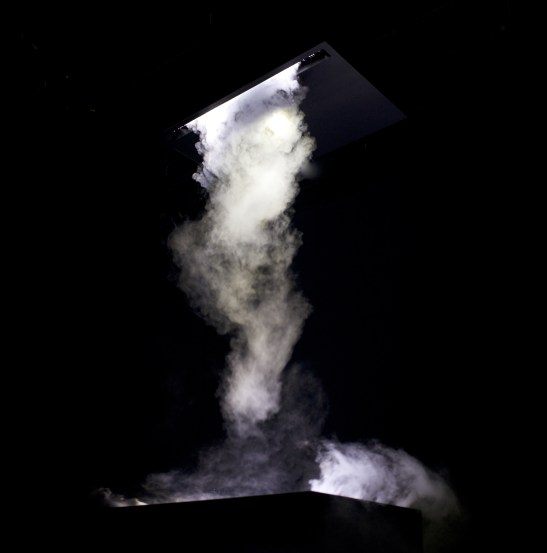
\includegraphics[width=0.8\textwidth]{images/tumbleweed.jpg}
\end{frame}

\begin{frame}
\centering
\Huge Pierre Cochard - Quarrè
\end{frame}

\begin{frame}
\centering
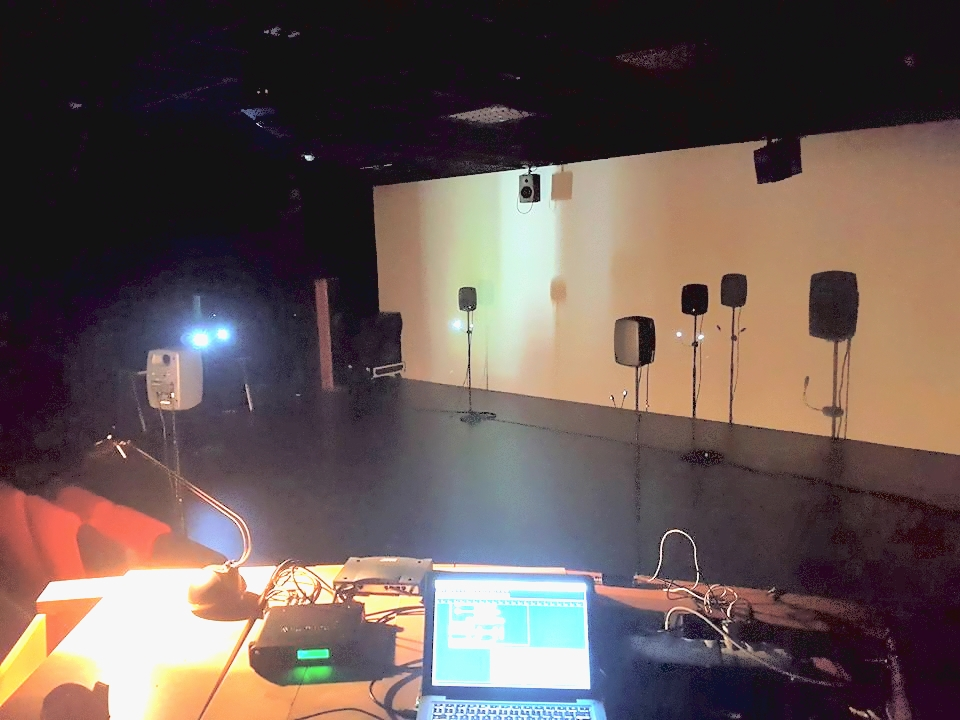
\includegraphics[width=\textwidth]{images/quarre.jpg}
\end{frame}

\begin{frame}
\centering
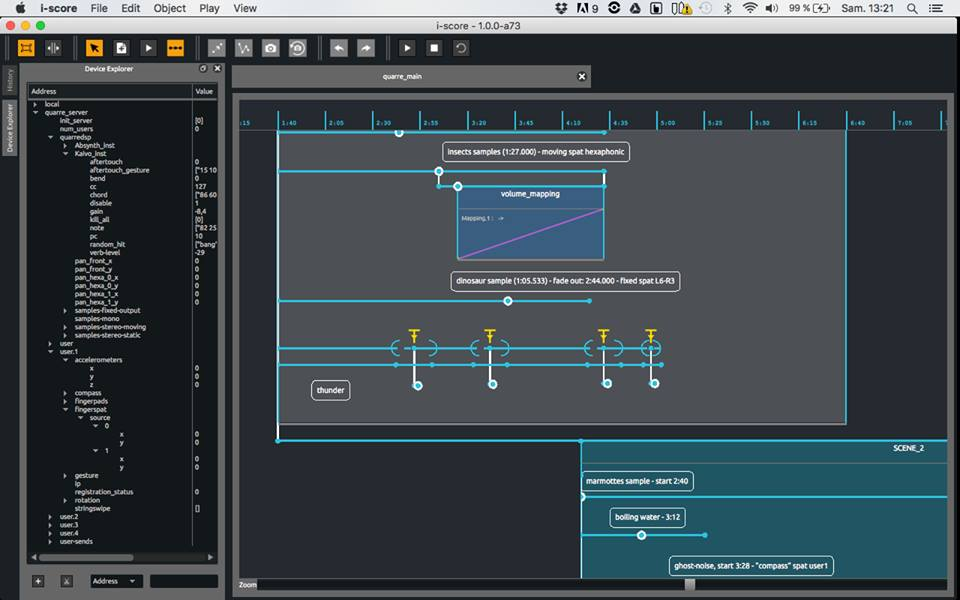
\includegraphics[width=\textwidth]{images/quarre-2.jpg}
\end{frame}

\begin{frame}
\centering
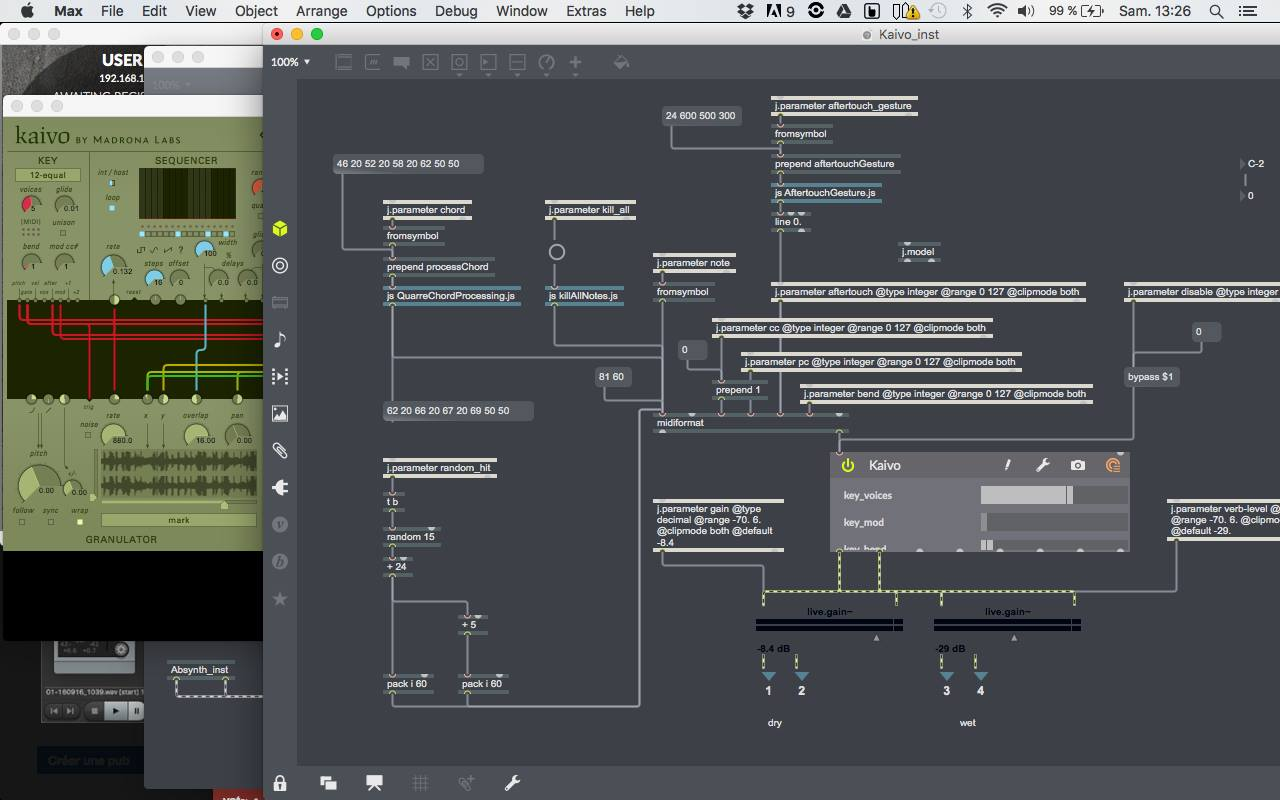
\includegraphics[width=\textwidth]{images/quarre-3.jpg}
\end{frame}

\begin{frame}
\Large
\begin{itemize}
    \item Digital arts: music, video, transmedia, etc...
    \item Temporal structure \& interactivity.
    \item Interoperability: software, hardware.
\end{itemize}
\end{frame}

\begin{frame}
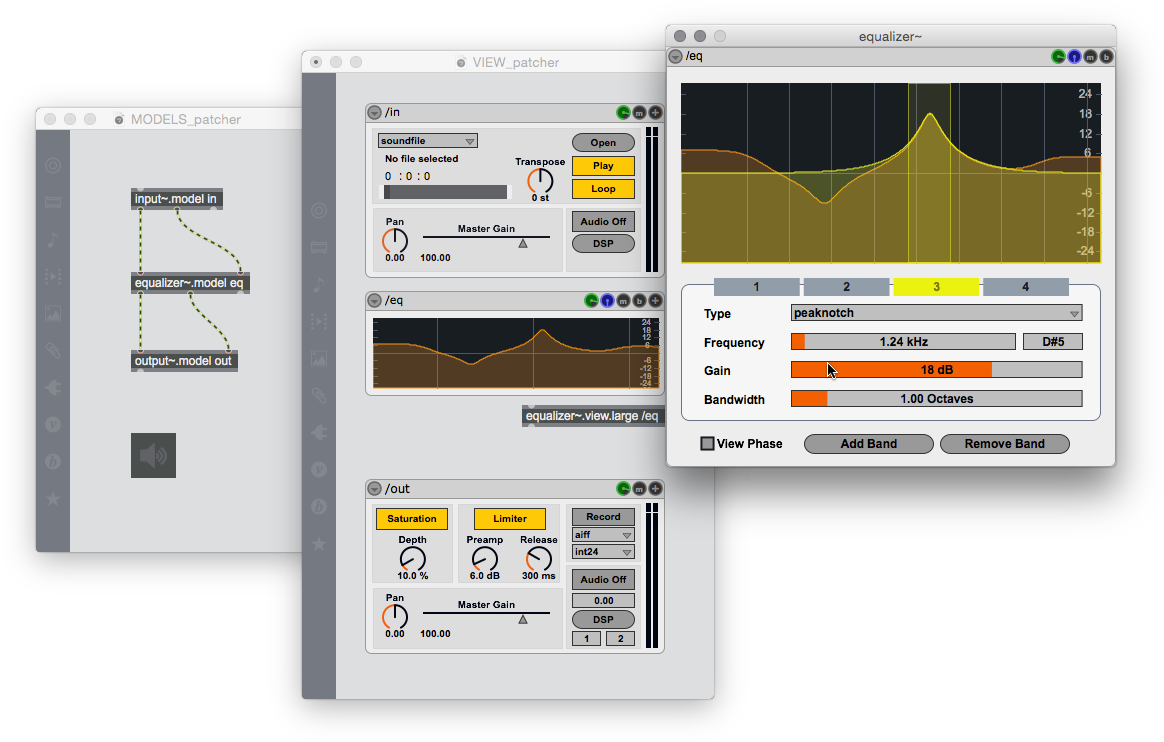
\includegraphics[width=\textwidth]{images/jamoma.jpg}
\end{frame}



\section{Foundation: libossia}
\subsection{Goal}

\begin{frame}
\frametitle{libossia: goals}
\Large
\begin{itemize}
    \item Automatic discovery.
    \item Shared object model inspired from OSC.
    \item Scoring primitives.
\end{itemize}
\end{frame}

\subsection{Protocols}
\begin{frame}
\frametitle{libossia: protocols}
\Large
\begin{itemize}
    \item{OSC}
    \item{Minuit}
    \item{OSCQuery}
    \item{MIDI}
    \item{HTTP (Requires Qt)}
    \item{WebSocket (Requires Qt)}
    \item{Serial port (Requires Qt)}
\end{itemize}

To come: ArtNet (DMX)
\end{frame}

\begin{frame}
\frametitle{Standard protocols}
\Large

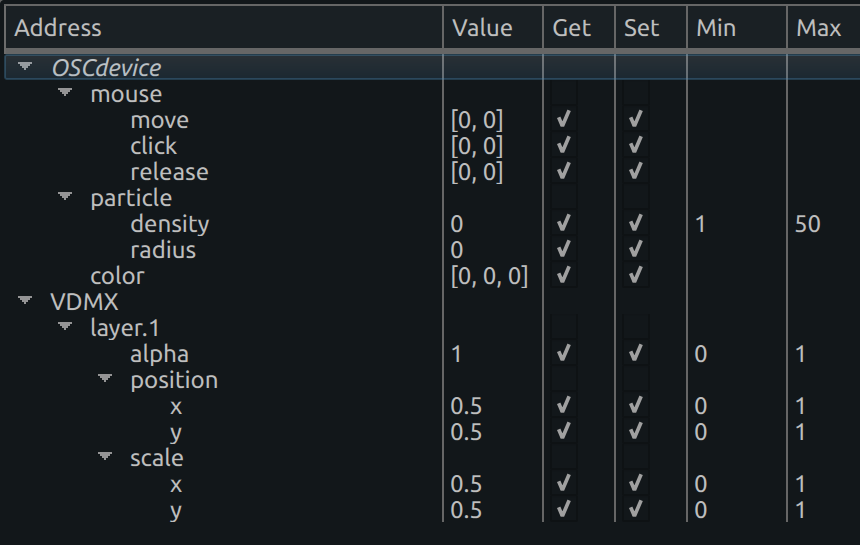
\includegraphics[width=\textwidth]{images/tree.png}
\end{frame}


\begin{frame}[fragile]
\frametitle{Qt-based protocols}
\Large
When no tree structure easily makes sense,~\\let the user script it !
\footnotesize
\begin{lstlisting}
function onMessage(message) {
    console.log(message);
    var res = JSON.parse(message);
    console.log(res.value);
    if(res.name === "toto")
    {
        return [ { address: "/toto", value: res.value } ];
    }
    return { };
}

function createTree() {
    return [ {
                name: "tata",
                children: [
                    {
                        name: "tutu",
                        request: "{ \"name\": \"toto\", \"value\": $val }",
                        type: Ossia.Float,
                        unit: "color.rgb"
                    },
\end{lstlisting}
\end{frame}

\subsection{Interoperability}

\begin{frame}[fragile]
\frametitle{libossia (C++14)}
Linux, macOS, Windows, GCC, Clang, MSVC, static, dynamic\dots
~\\
Only header-only dependencies.

~\\
\footnotesize
\begin{lstlisting}[language=C++]
auto& node = find_or_create_node(device, "/test/my_int");
auto address = node.create_address(val_type::INT);

node.set(access_mode_attribute{}, access_mode::GET);
node.set(bounding_mode_attribute{}, bounding_mode::FOLD);
node.set(domain_attribute{}, make_domain(2, 14));
node.set(description_attribute{}, "an integral value");

address->add_callback([] (const auto& val) {
    std::cout << val << " ";
  });

address->push_value(5678);
\end{lstlisting}
\end{frame}

\begin{frame}[fragile]
\frametitle{ofxOssia}
\Large Integration with ofParameter, ofParameterGroup
~\\
\footnotesize
\begin{lstlisting}[language=C++]
ossia::Parameter<bool> _fill;
ossia::Parameter<ofColor> _color;
ossia::ParameterGroup _sizeParams;
...
_circleParams.setup(_parent_node, "circle");

_sizeParams.setup(_circleParams, "sizeParams");
_radius.setup(_sizeParams,"radius",10.,1.,100.);
_position.setup(_sizeParams,
                "position",
                ofVec2f(ofGetWidth() / 2, ofGetHeight() / 2),
                ofVec2f(0., 0.), // Min
                ofVec2f(ofGetWidth(), ofGetHeight())); // Max
\end{lstlisting}
\end{frame}

\begin{frame}
\frametitle{ossia-pd (and ossia-max soon)}
\Large
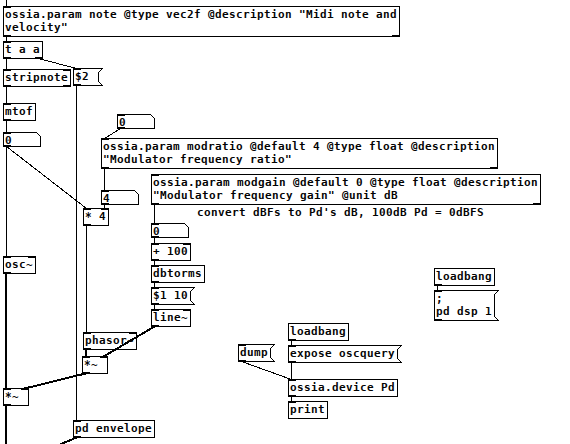
\includegraphics[width=\textwidth]{images/ossiapd.png}
\end{frame}

\begin{frame}[fragile]
\frametitle{ossia-python}
\footnotesize
\begin{lstlisting}[language=python]
# create a node, create a tuple address and initialize it
tuple_node = local_device.add_node("/test/value/tuple")
tuple_address = tuple_node.create_address(
                    ossia.ValueType.Tuple)
tuple_value = ossia.Value([
    ossia.Value(44100),
    ossia.Value("test.wav"),
    ossia.Value(0.9)]
    )
tuple_address.push_value(tuple_value)

# attach a callback function to the boolean address
def bool_value_callback(v):
    print(v.get())
    bool_address.add_callback(bool_value_callback)
\end{lstlisting}
\end{frame}

\begin{frame}[fragile]
\frametitle{ossia-unity3D (C\#)}
\Large
\footnotesize
\begin{lstlisting}[language=python]
public class Foo : public MonoBehaviour
{
  [Ossia.Attribute]
  int foo;
}
\end{lstlisting}
\end{frame}

\begin{frame}[fragile]
\frametitle{ossia-qml (Qt QML)}
\small
\begin{lstlisting}
Item {
  Ossia.Node { name: 'test' }
  AngleSlider {
    // Reads and writes from /test/angle
    Ossia.Property on angle {
      min: -90
      max: 0
      bounding: Ossia.Context.Clip
    }
  }
}
\end{lstlisting}
% controls
% video, shaders
\end{frame}

\begin{frame}[fragile]
\frametitle{ossia-C (C99)}
\small
\begin{lstlisting}[language=C]
OSSIA_EXPORT
bool ossia_device_update_namespace(
         ossia_device_t device);

OSSIA_EXPORT
ossia_node_t ossia_device_get_root_node(
         ossia_device_t device);

OSSIA_EXPORT
const char* ossia_device_get_name(
         ossia_device_t node);

//// Node ////
OSSIA_EXPORT
ossia_node_t ossia_node_add_child(
         ossia_node_t node,
         const char * name);
\end{lstlisting}
\end{frame}

\section{The sequencer: i-score}

\begin{frame}
\centering
\Huge Demonstration
~\\
~\\
\Large i-score + PureData + Processing
\end{frame}

\subsection{Control}

\begin{frame}
\frametitle{Sending messages}
\Large
\begin{figure}
    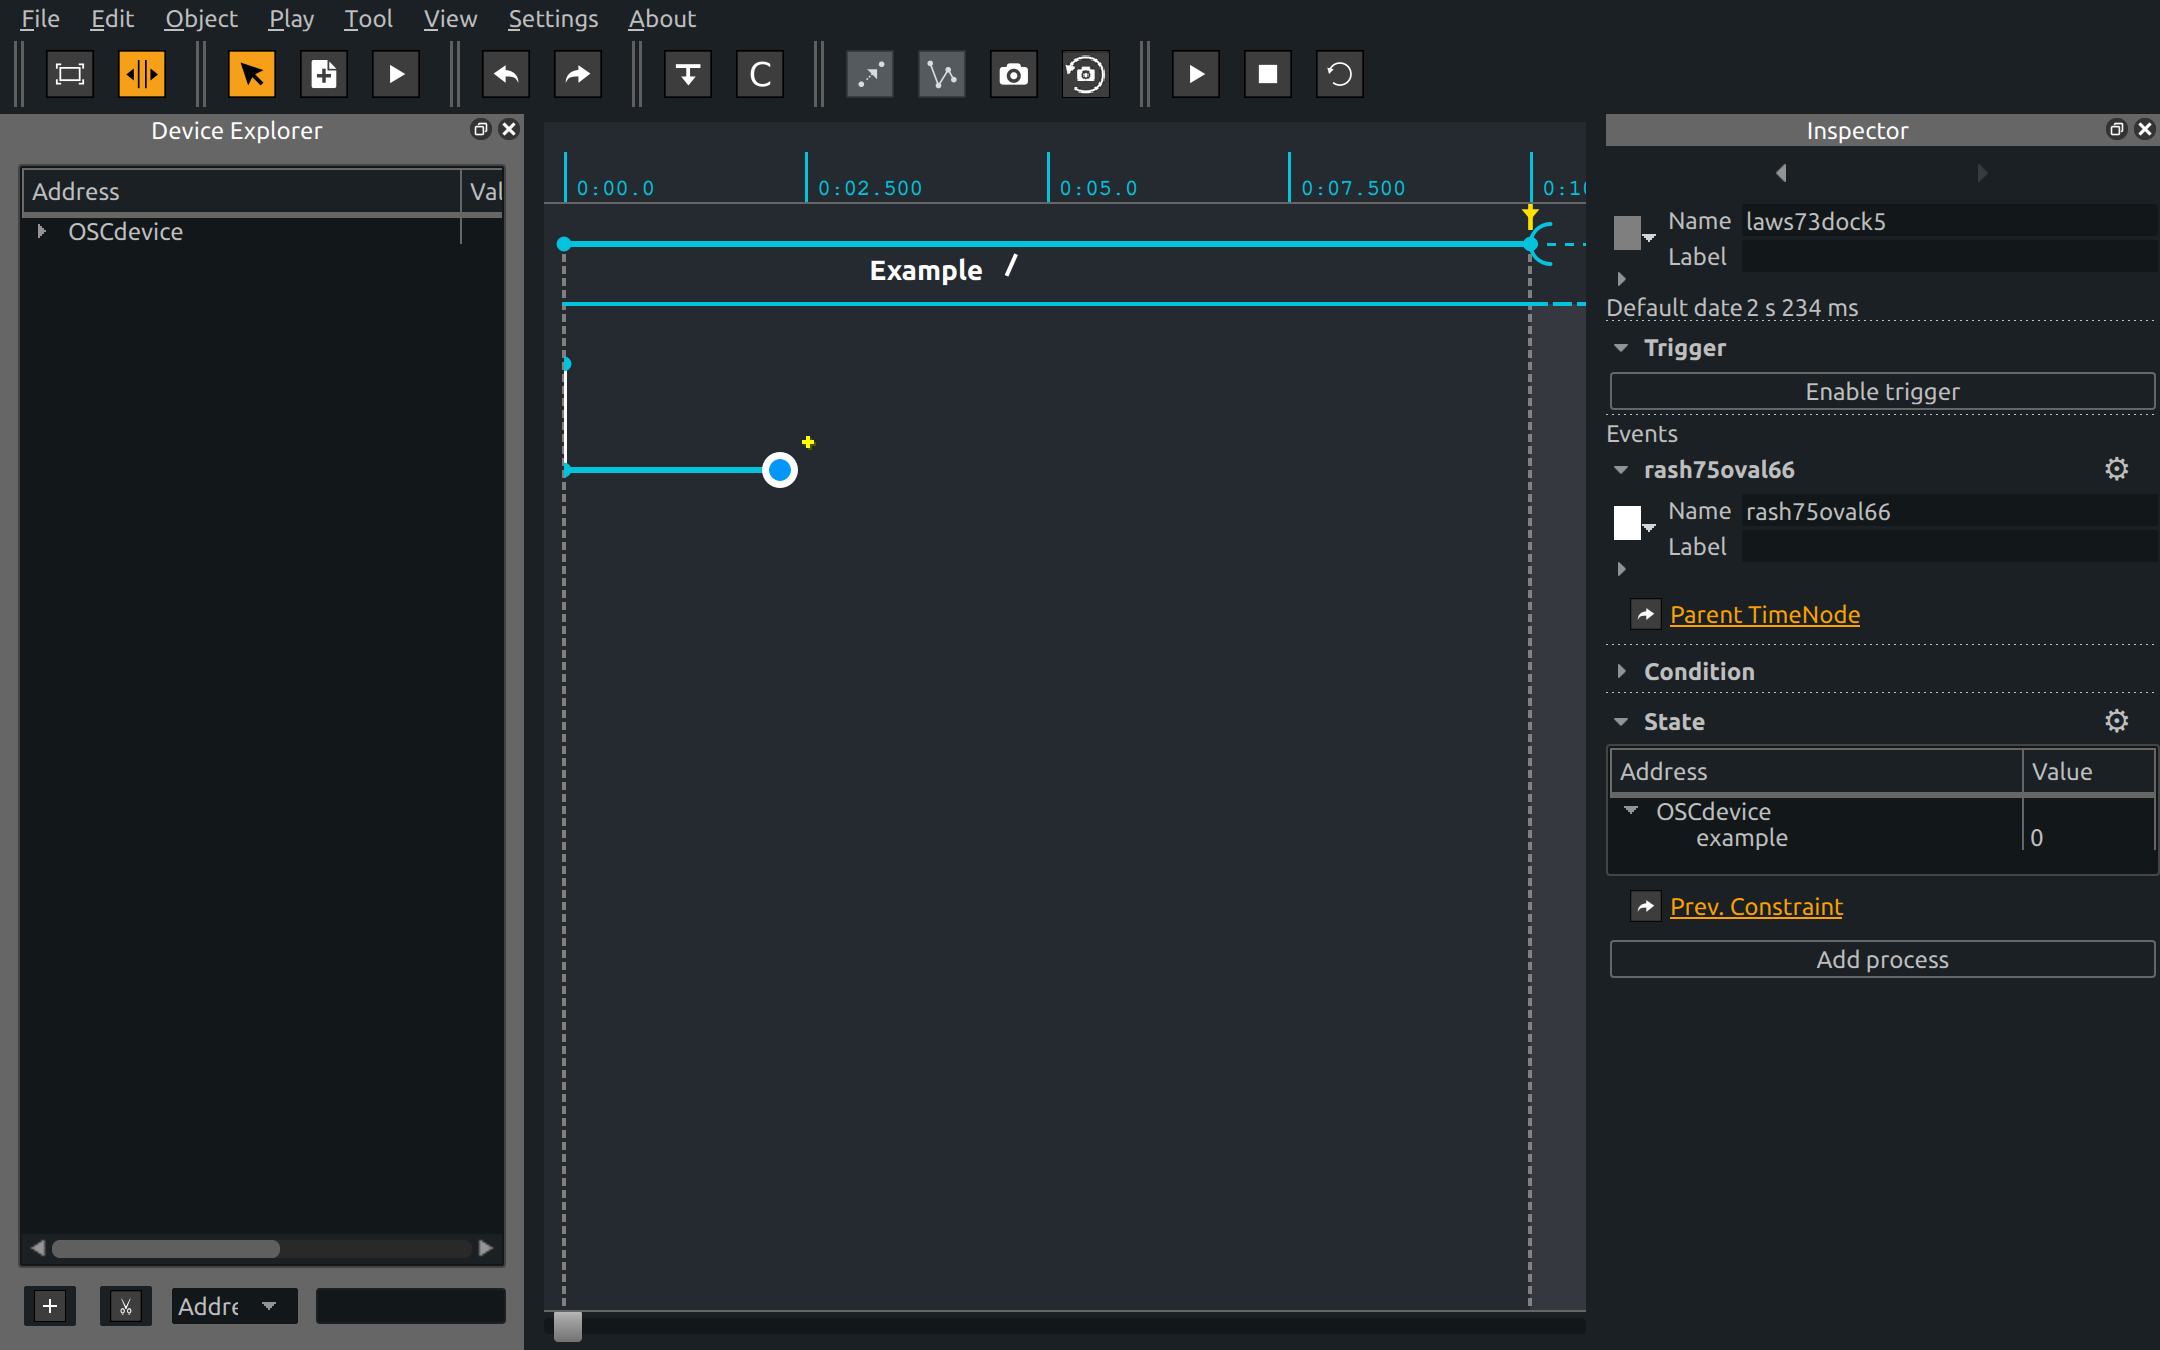
\includegraphics[width=\textwidth]{images/state.png}
\end{figure}
\end{frame}

\begin{frame}
\frametitle{Automating}
\Large
\begin{figure}
    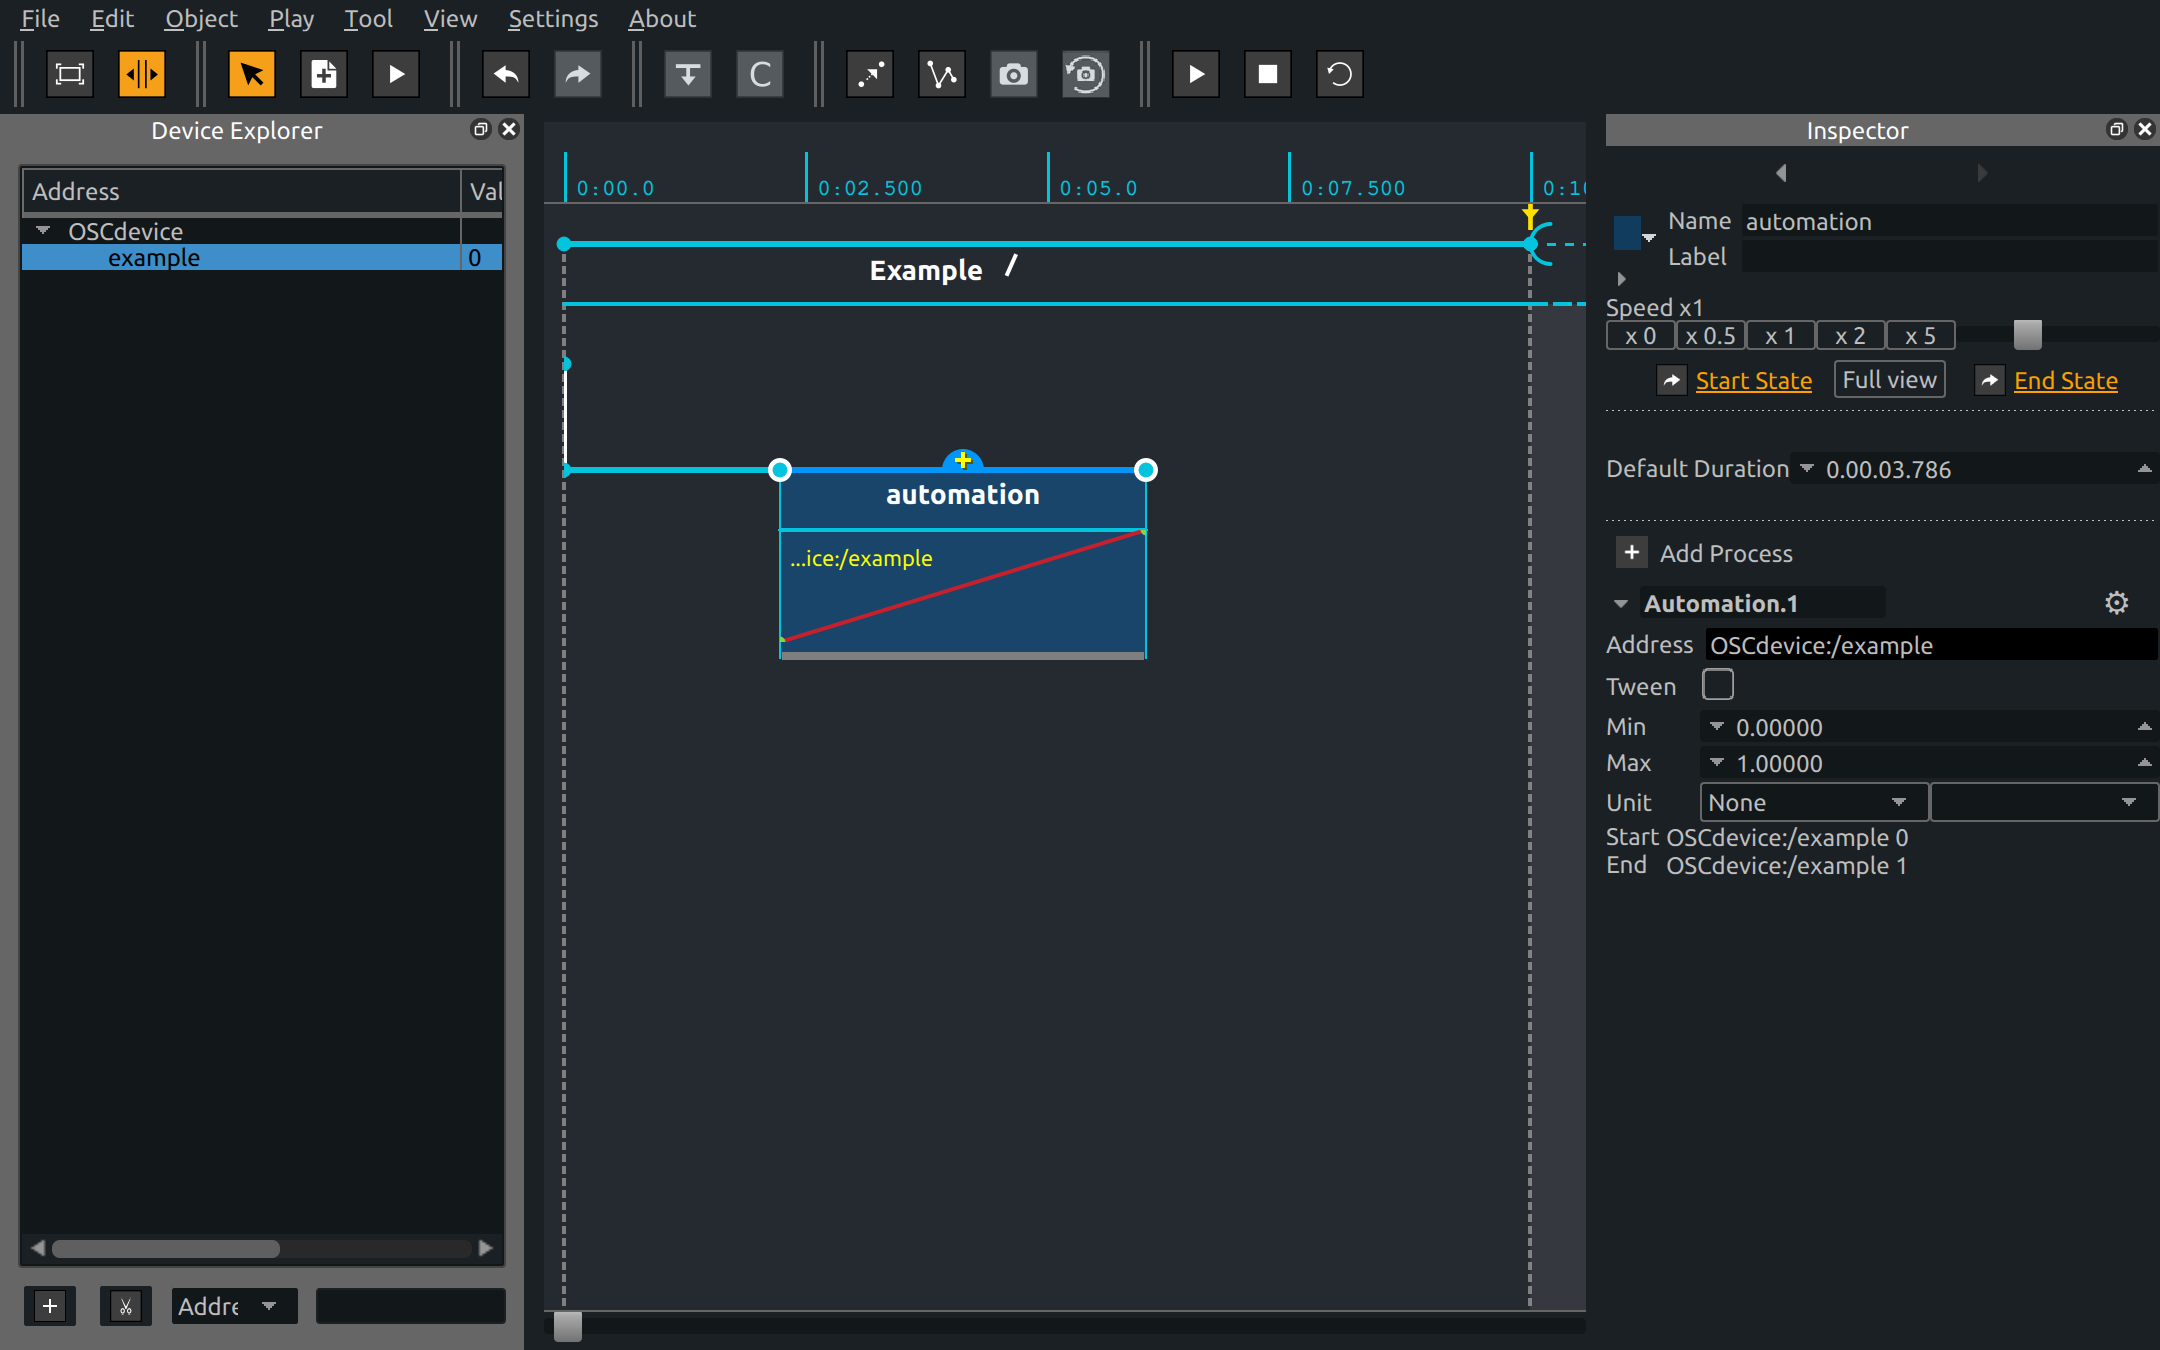
\includegraphics[width=\textwidth]{images/autom.png}
\end{figure}
\end{frame}

\begin{frame}
\frametitle{Interpolating}
\Large
\begin{figure}
    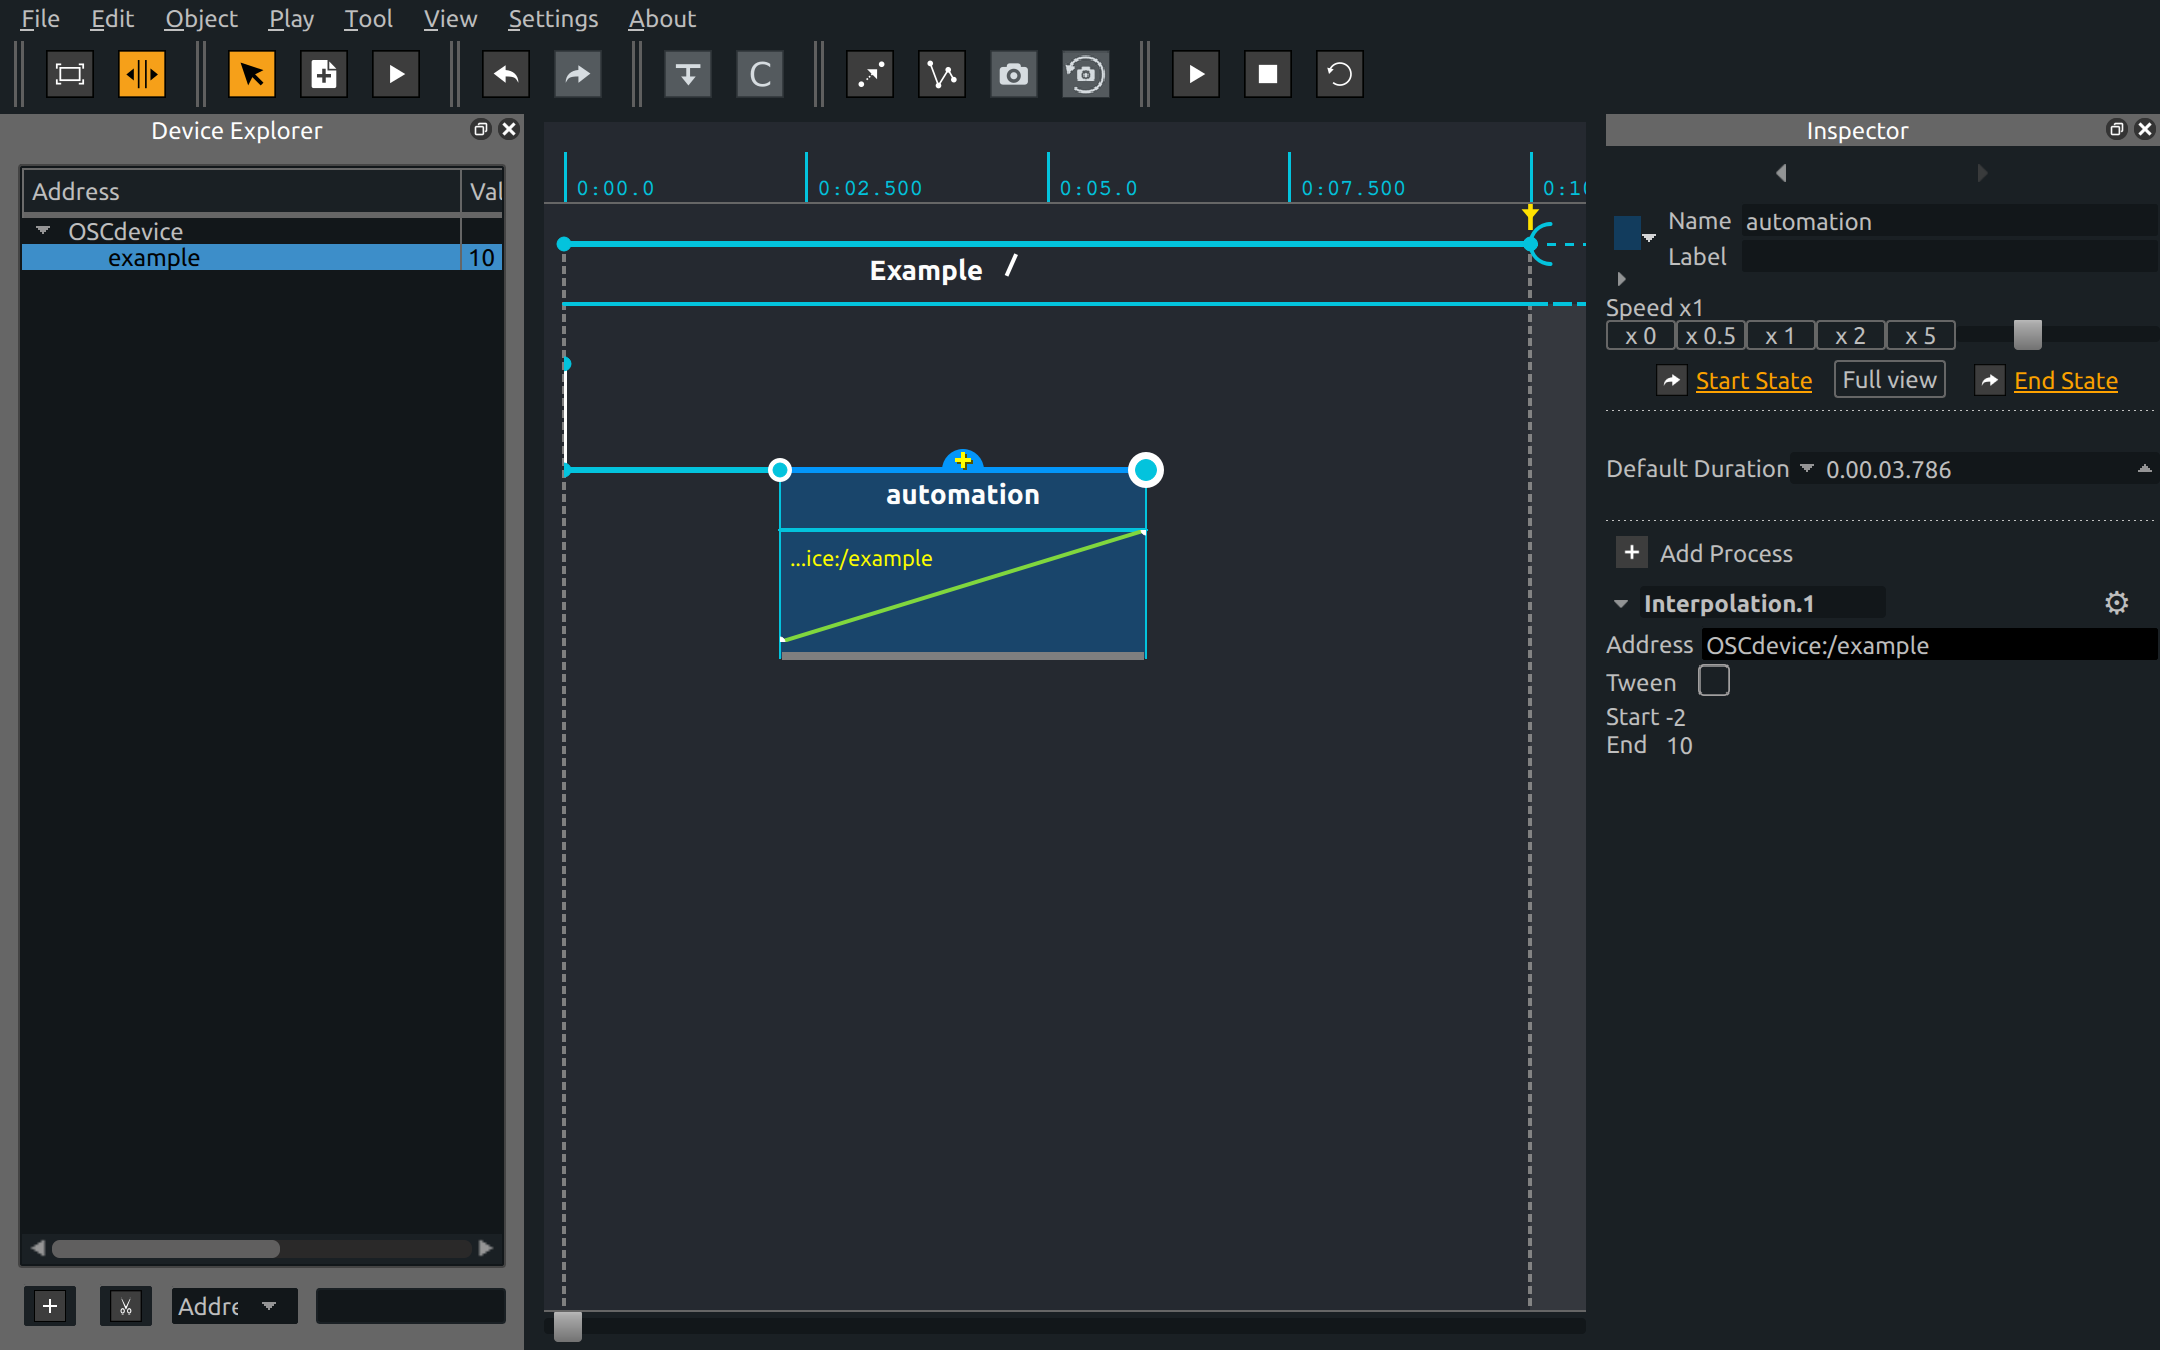
\includegraphics[width=\textwidth]{images/interp.png}
\end{figure}
\end{frame}

\begin{frame}
\frametitle{Tweening}
\Large
\begin{figure}
    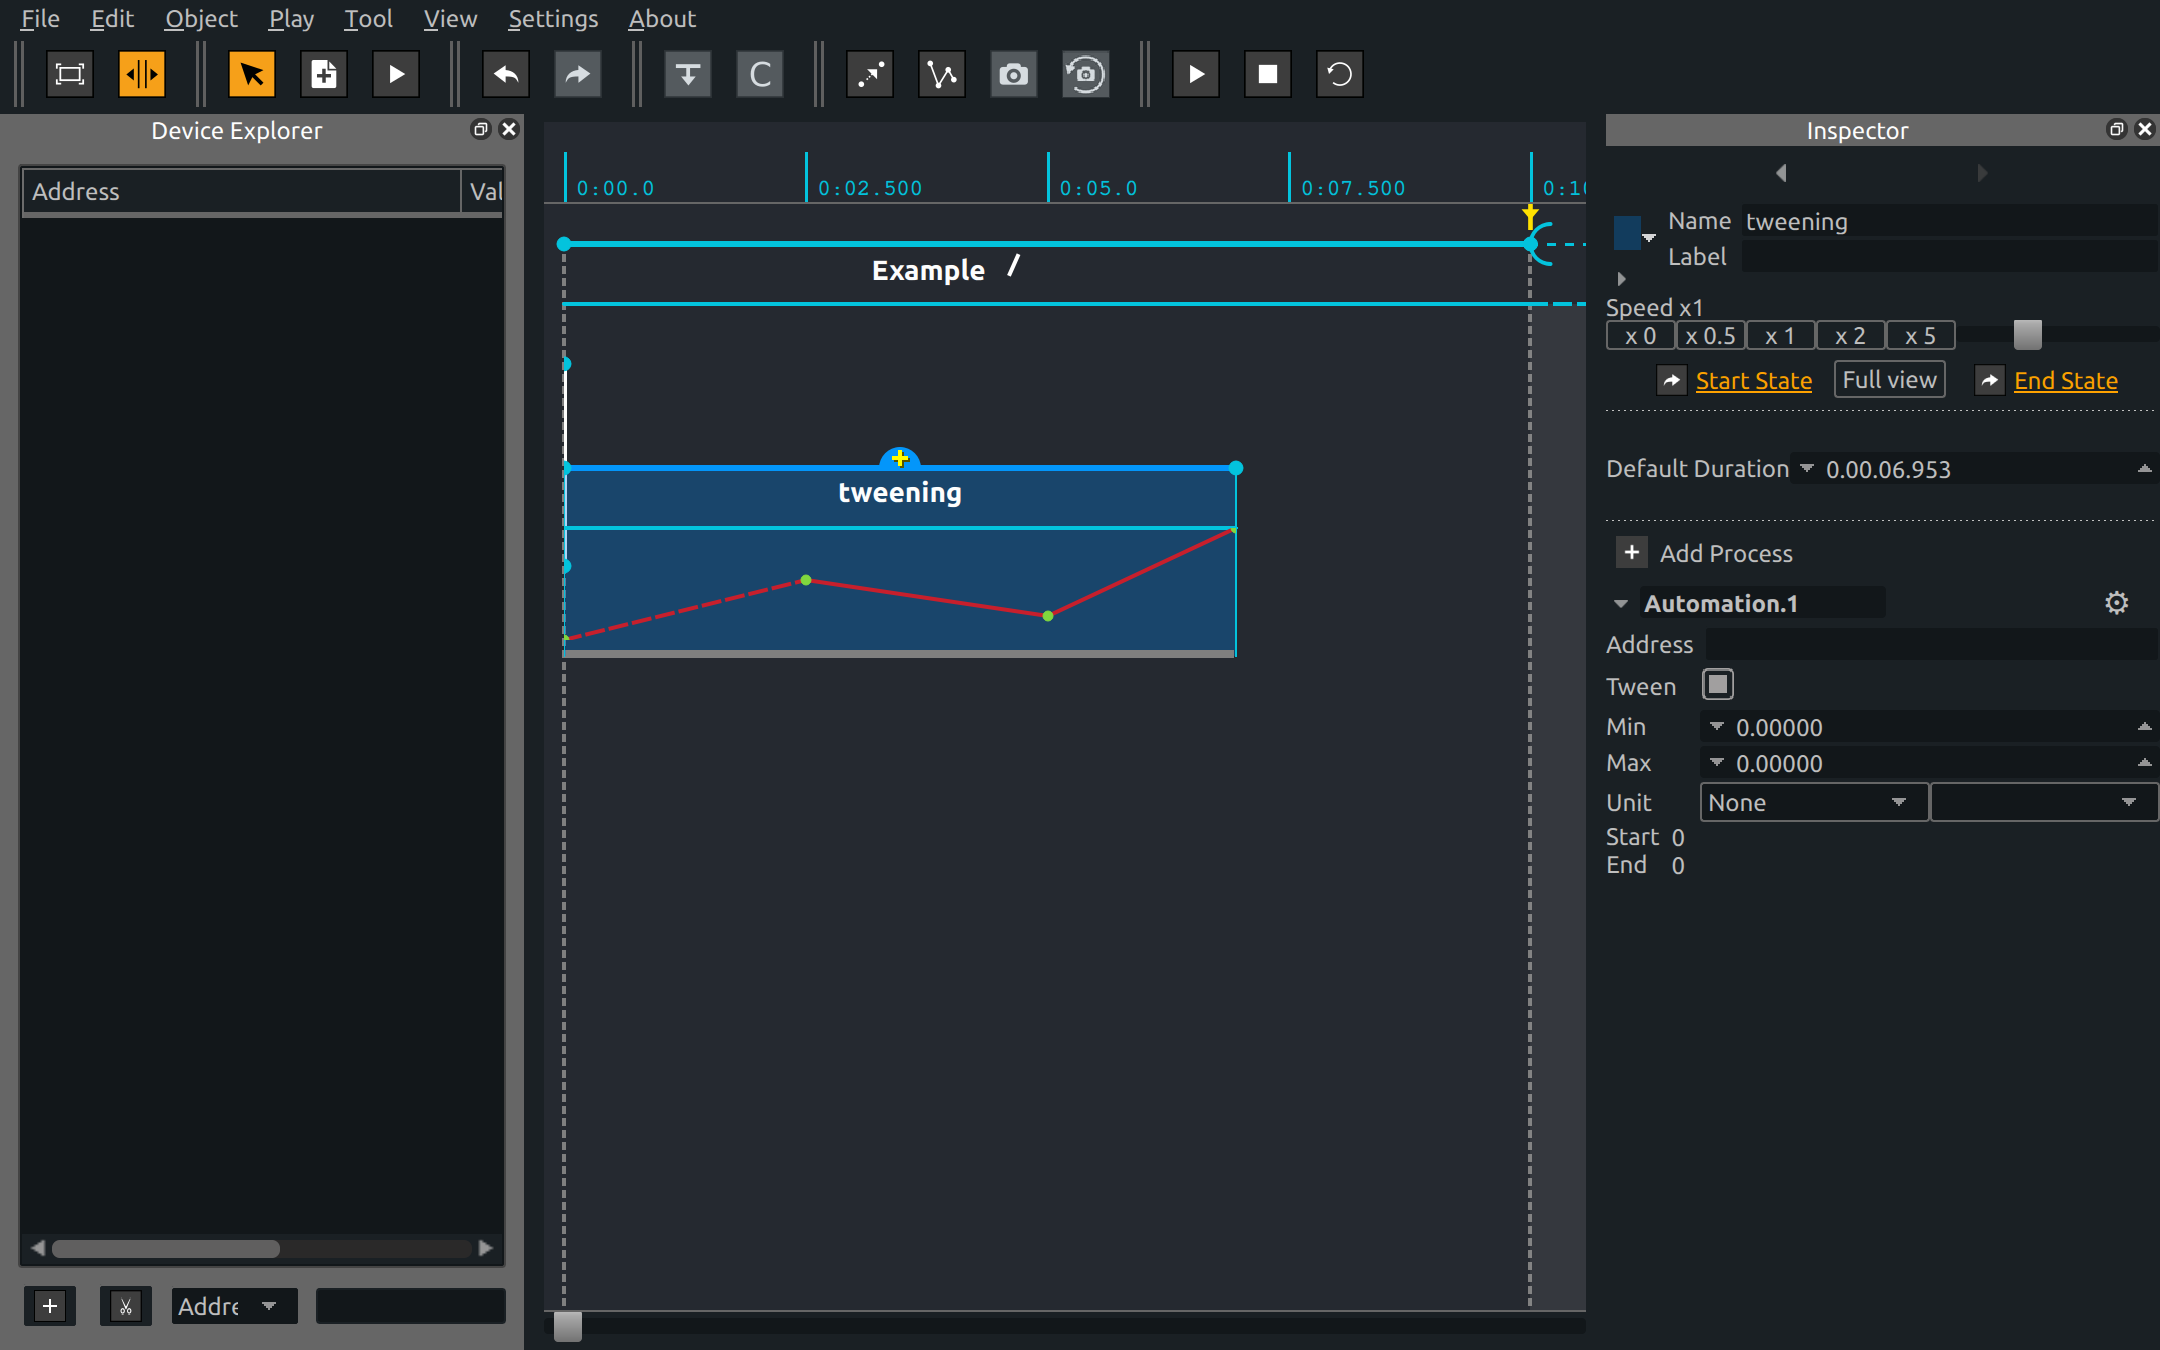
\includegraphics[width=\textwidth]{images/tween.png}
\end{figure}
\end{frame}

\begin{frame}
\frametitle{Mapping}
\Large
\begin{figure}
    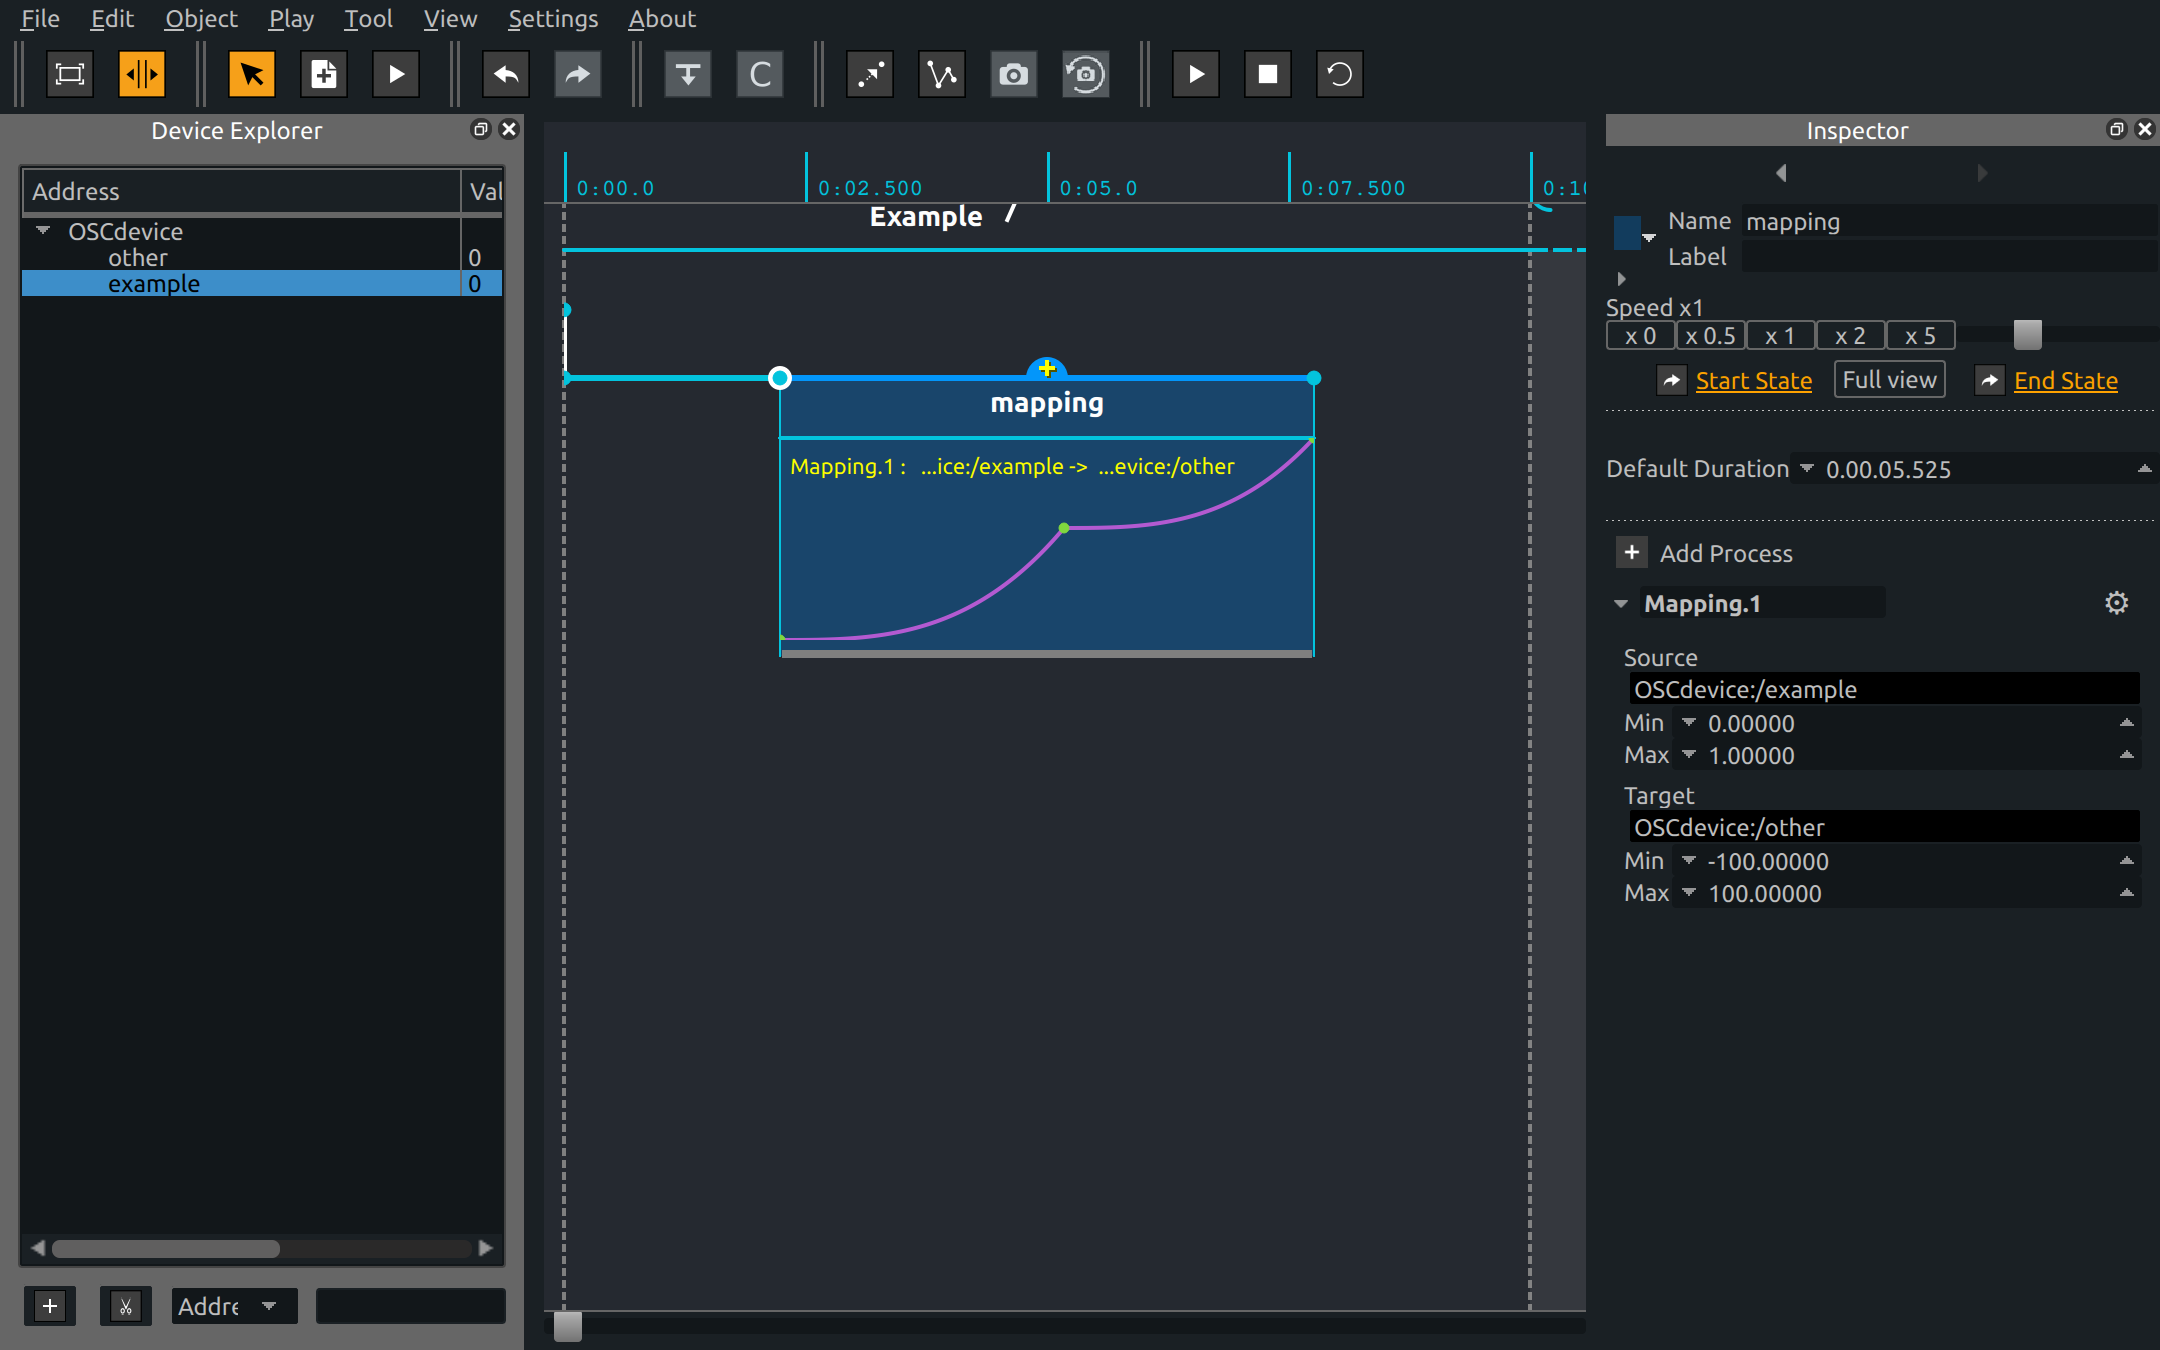
\includegraphics[width=\textwidth]{images/mapping.png}
\end{figure}
\end{frame}

\begin{frame}
\frametitle{Scripting}
\Large
\begin{figure}
    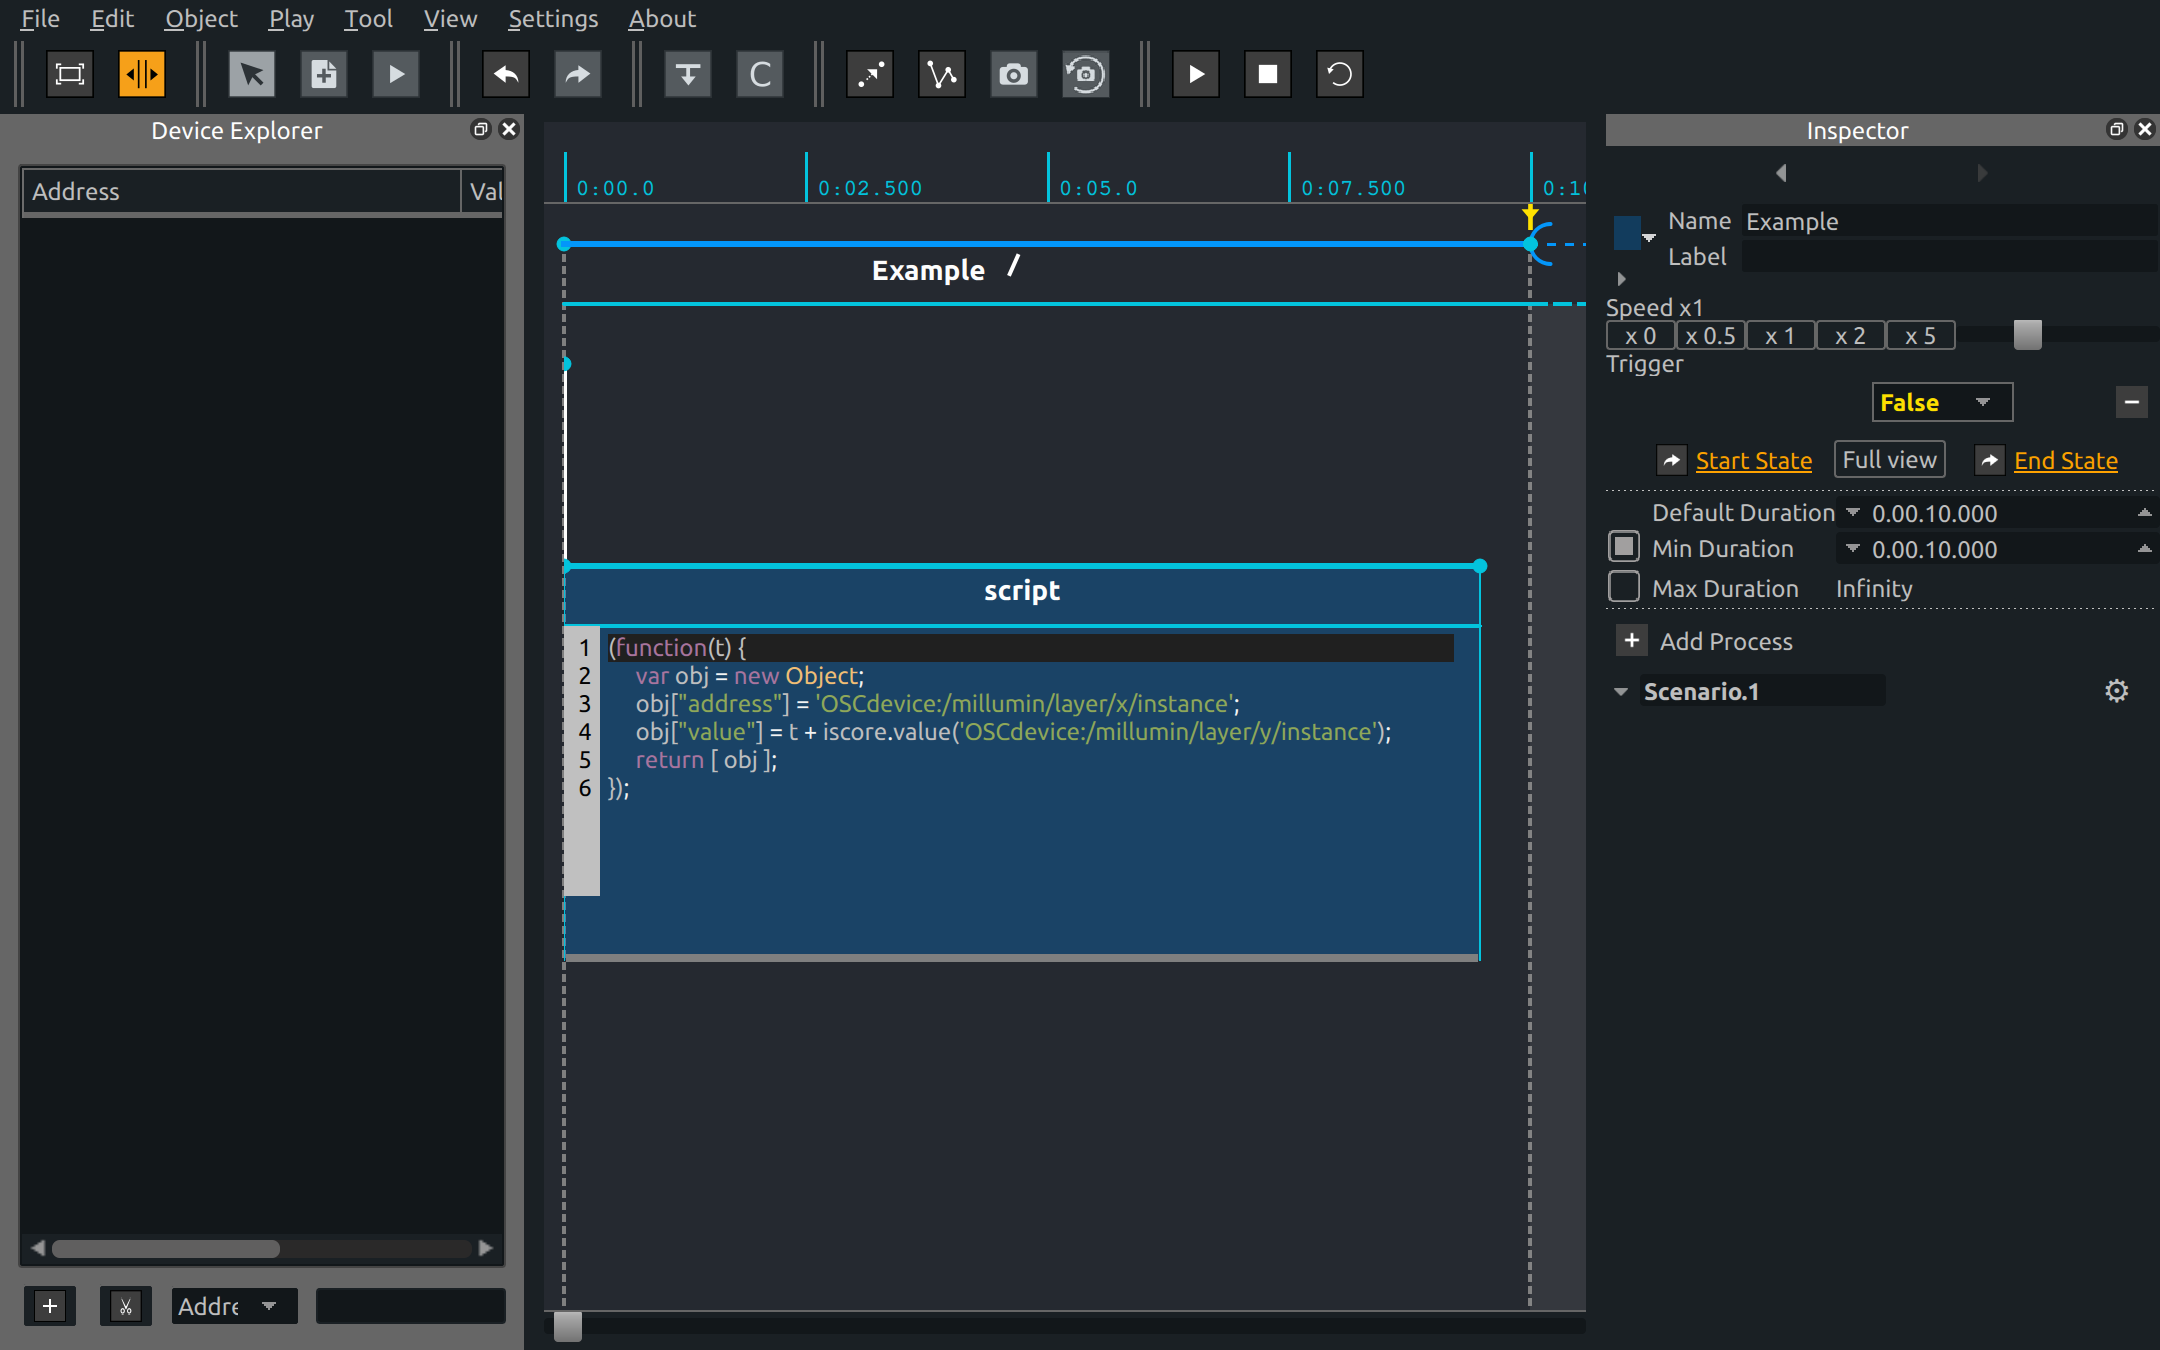
\includegraphics[width=\textwidth]{images/script.png}
\end{figure}
\end{frame}

\begin{frame}
\frametitle{Racks}
\Large
\begin{figure}
    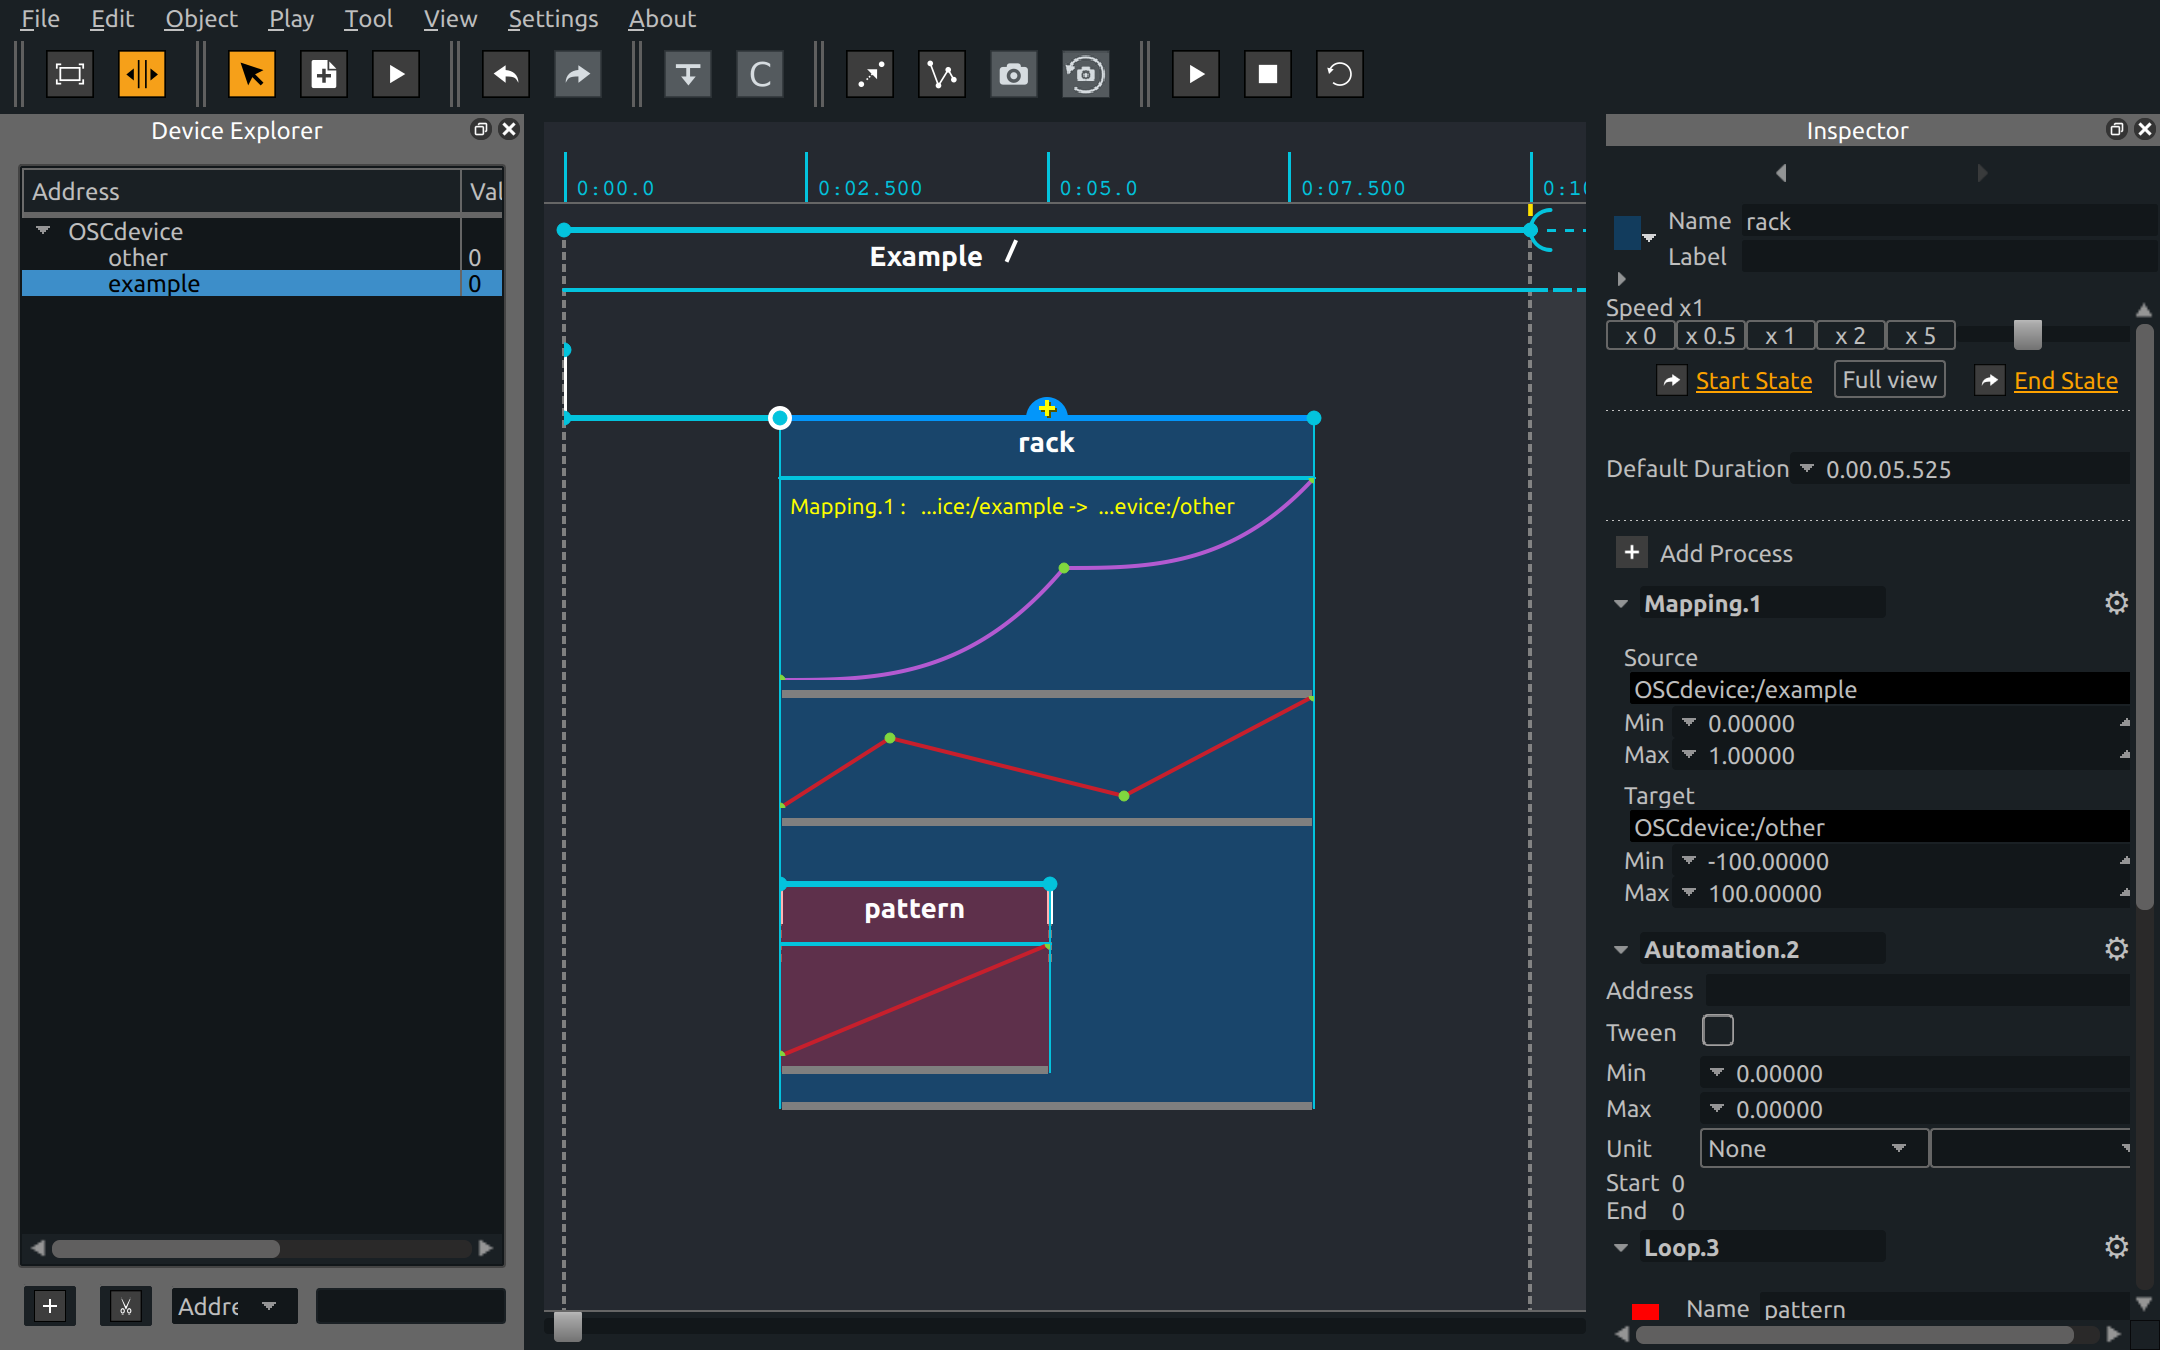
\includegraphics[width=\textwidth]{images/rack.png}
\end{figure}
\end{frame}

\subsection{Temporal structure}
\begin{frame}
\frametitle{Hierarchy}
\Large
\begin{figure}
    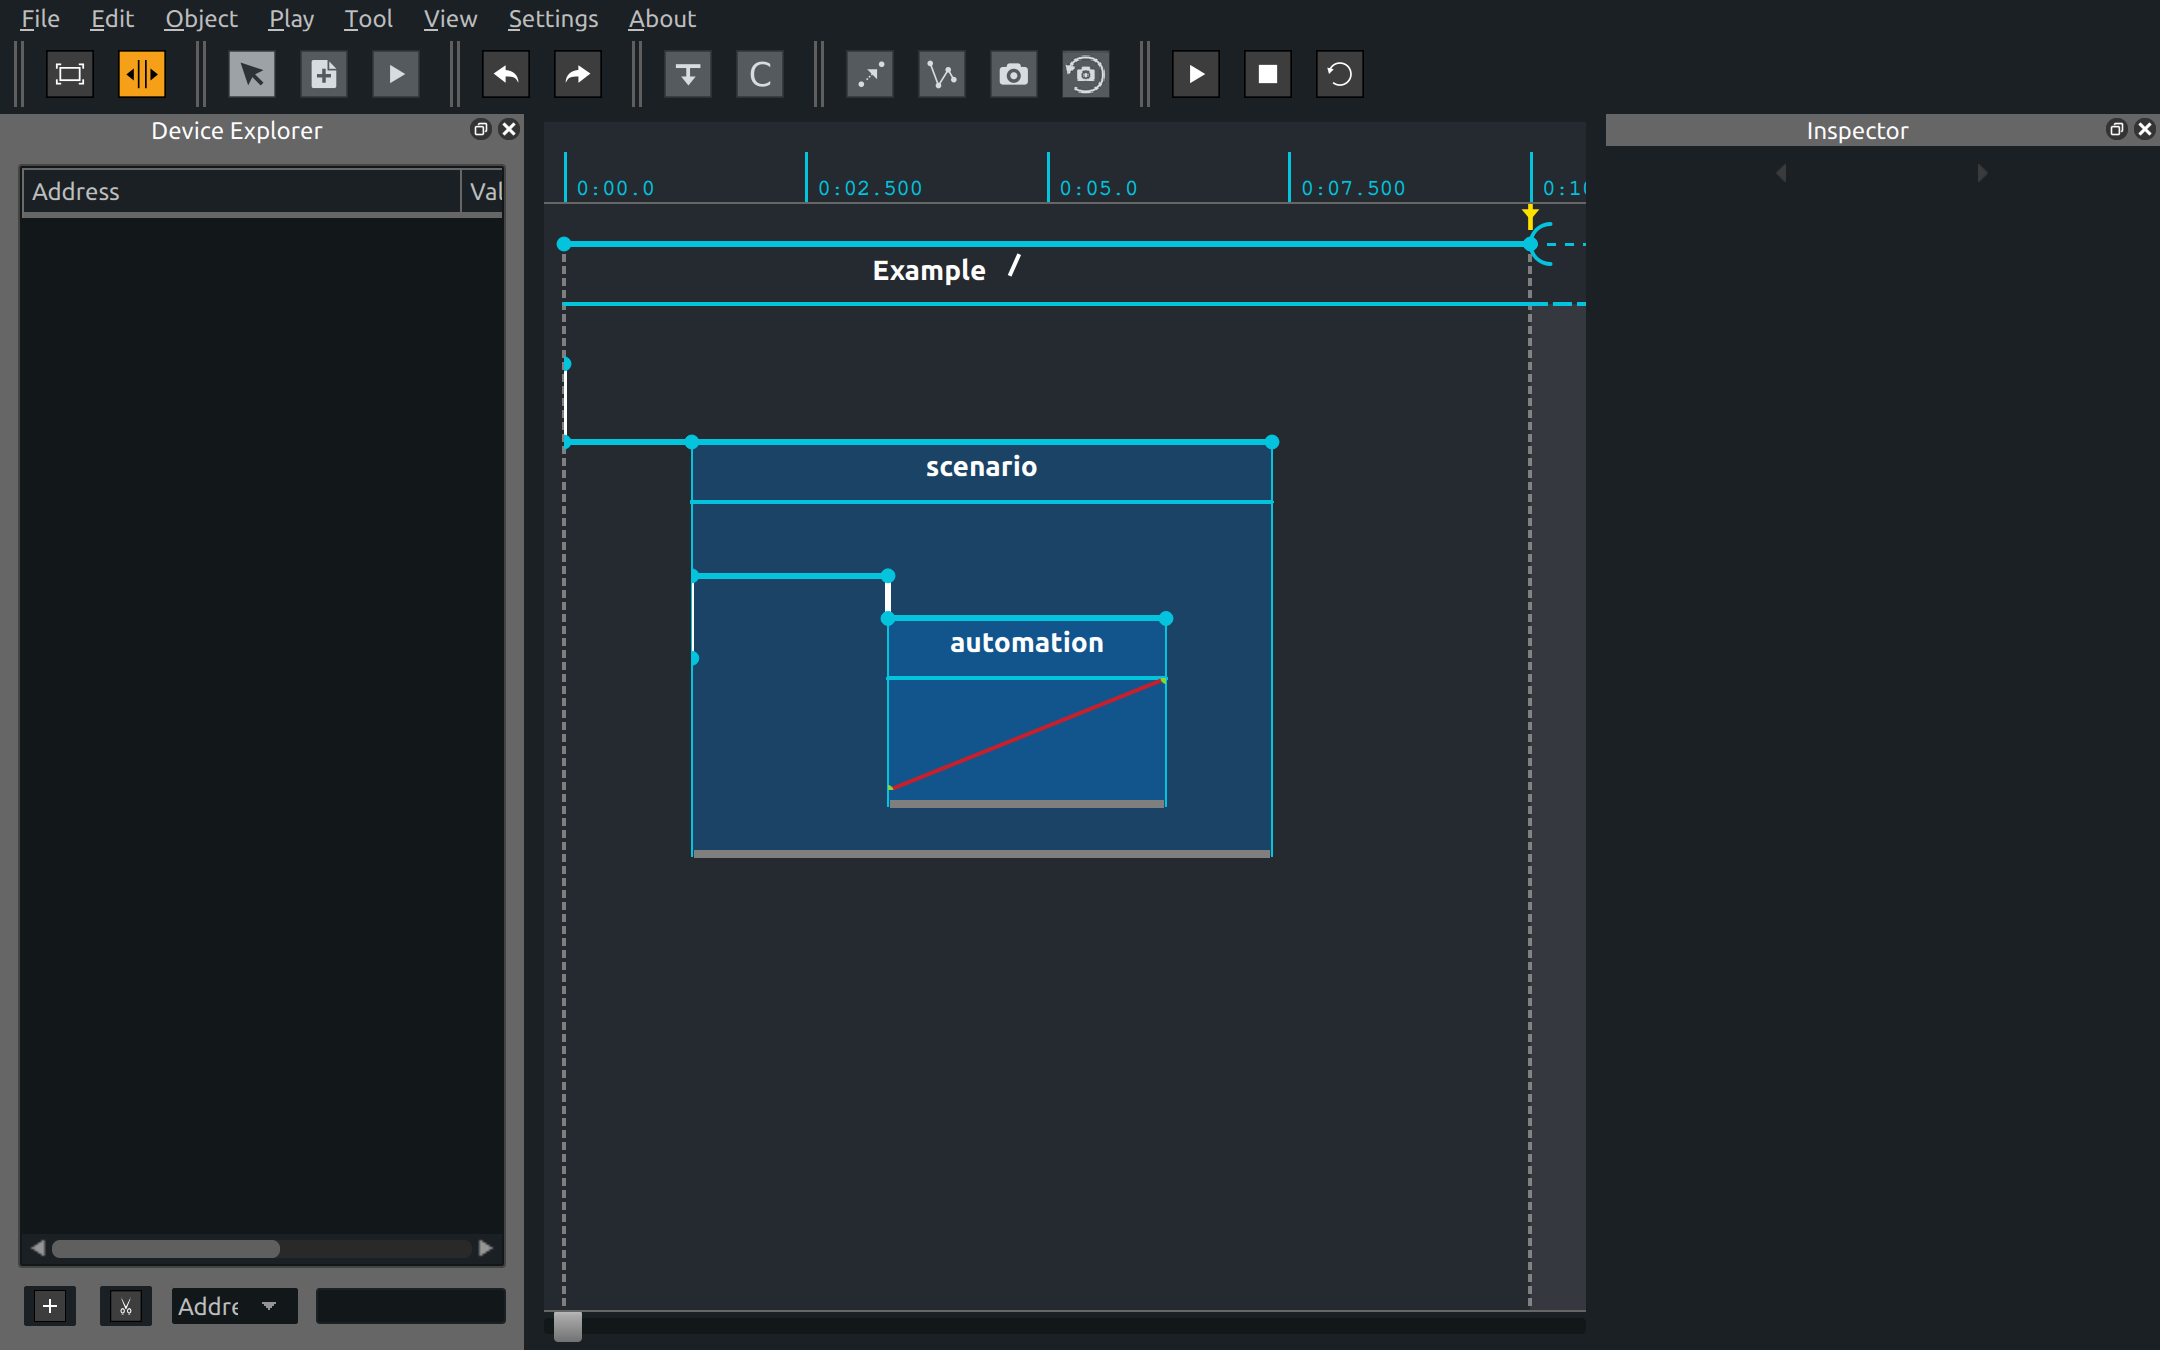
\includegraphics[width=\textwidth]{images/scenario.png}
\end{figure}
\end{frame}

\begin{frame}
\frametitle{Loops}
\Large
\begin{figure}
    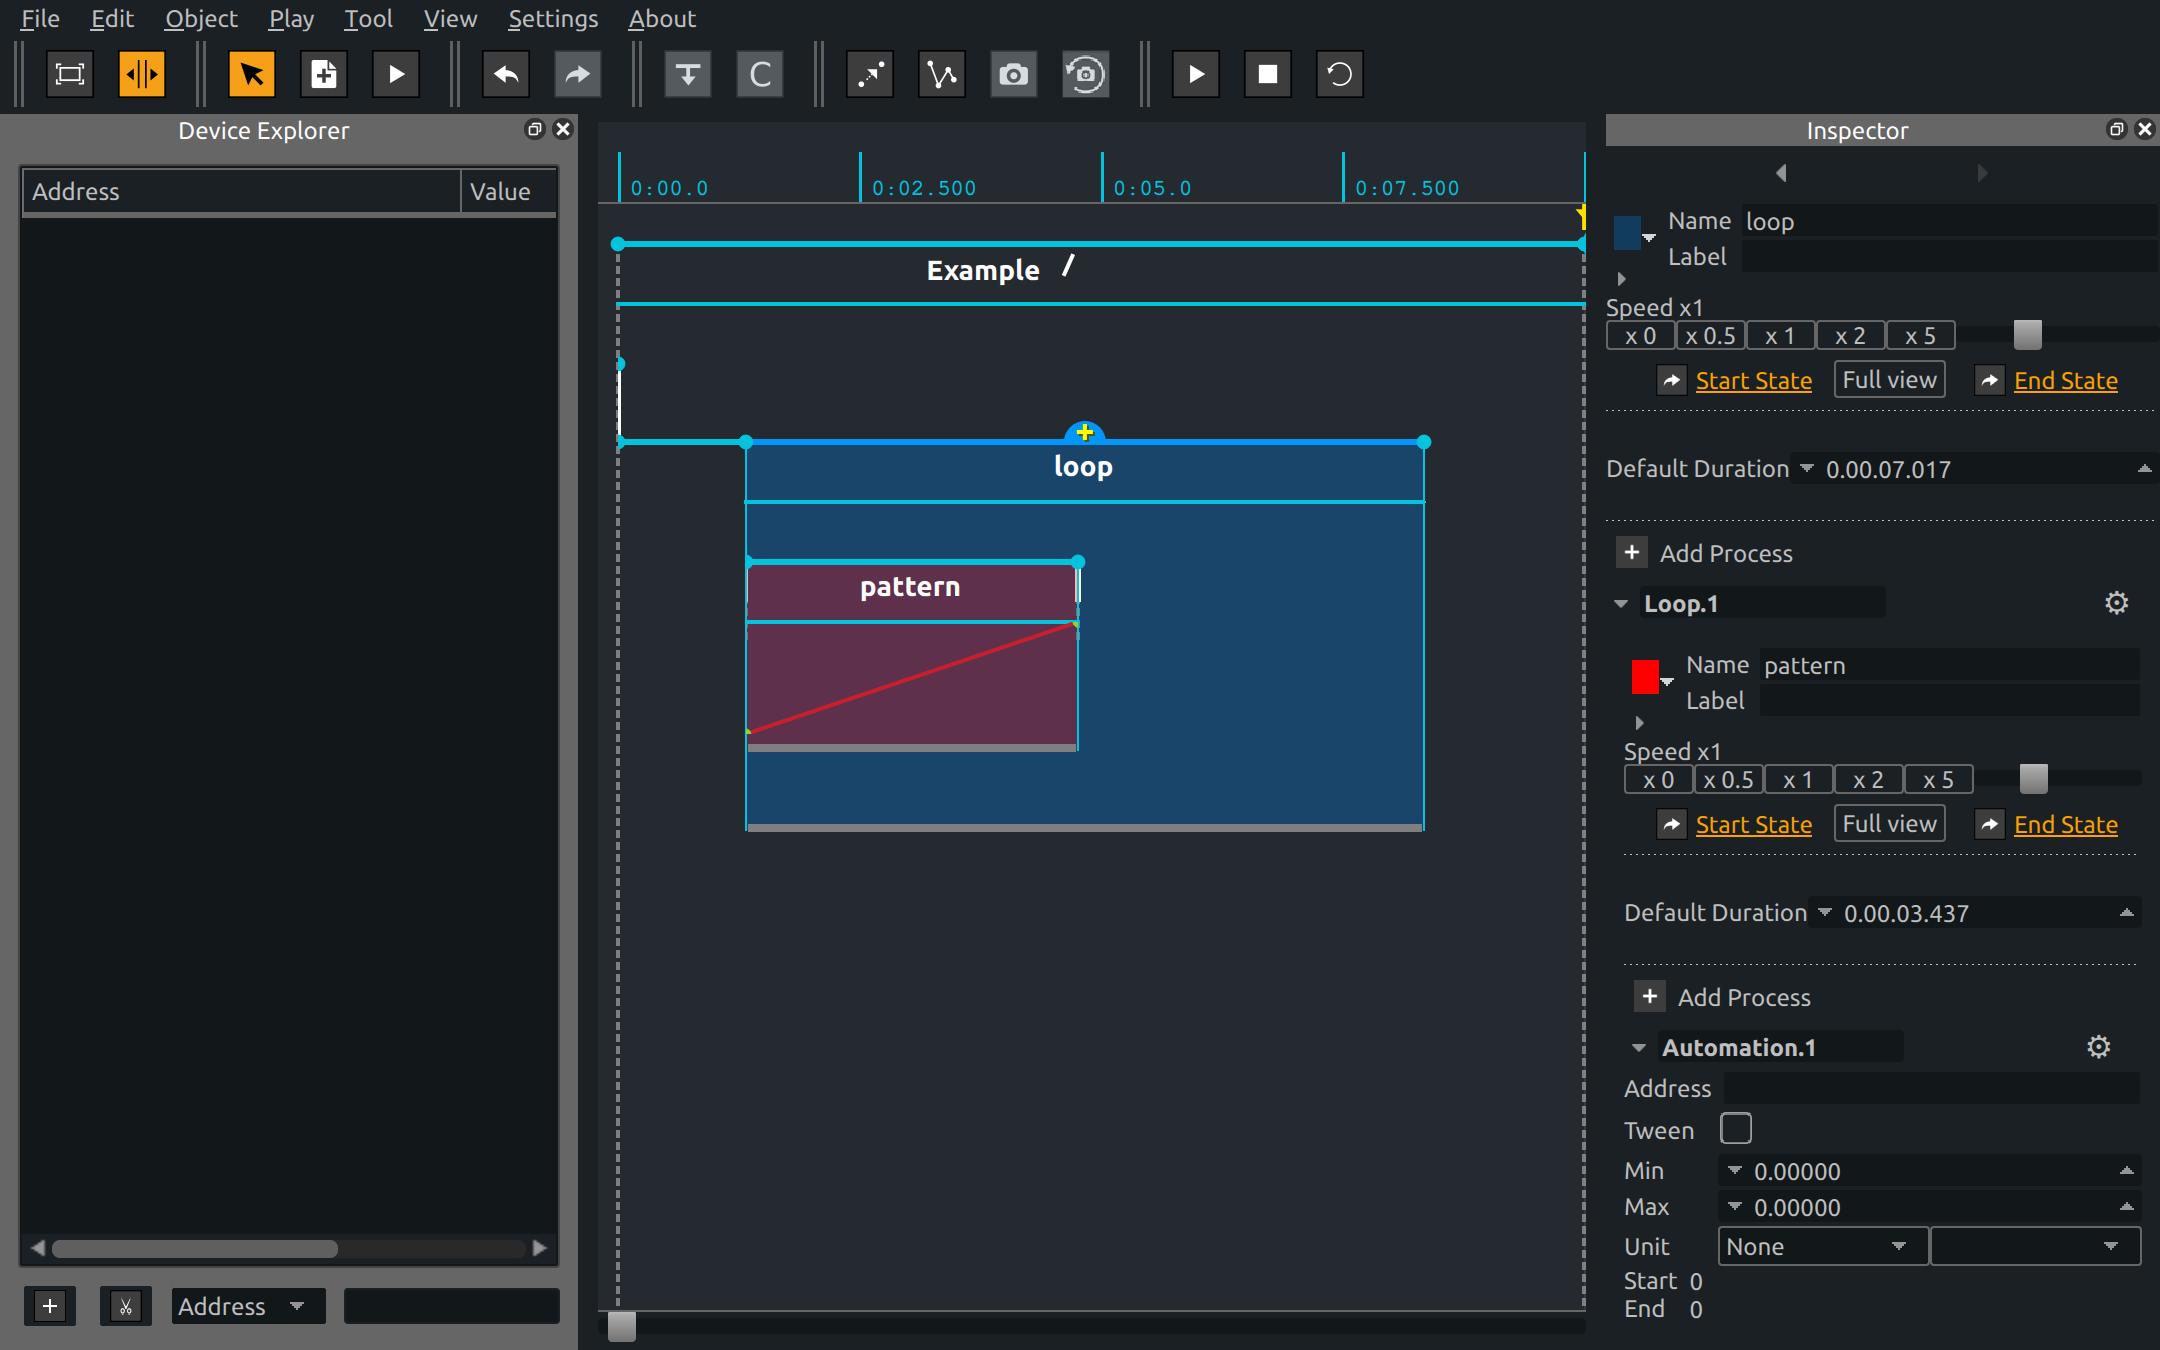
\includegraphics[width=\textwidth]{images/loop.png}
\end{figure}
\end{frame}

\subsection{Interactivity}
\begin{frame}
\frametitle{Interactivity: conditions}
\Large
\begin{figure}
    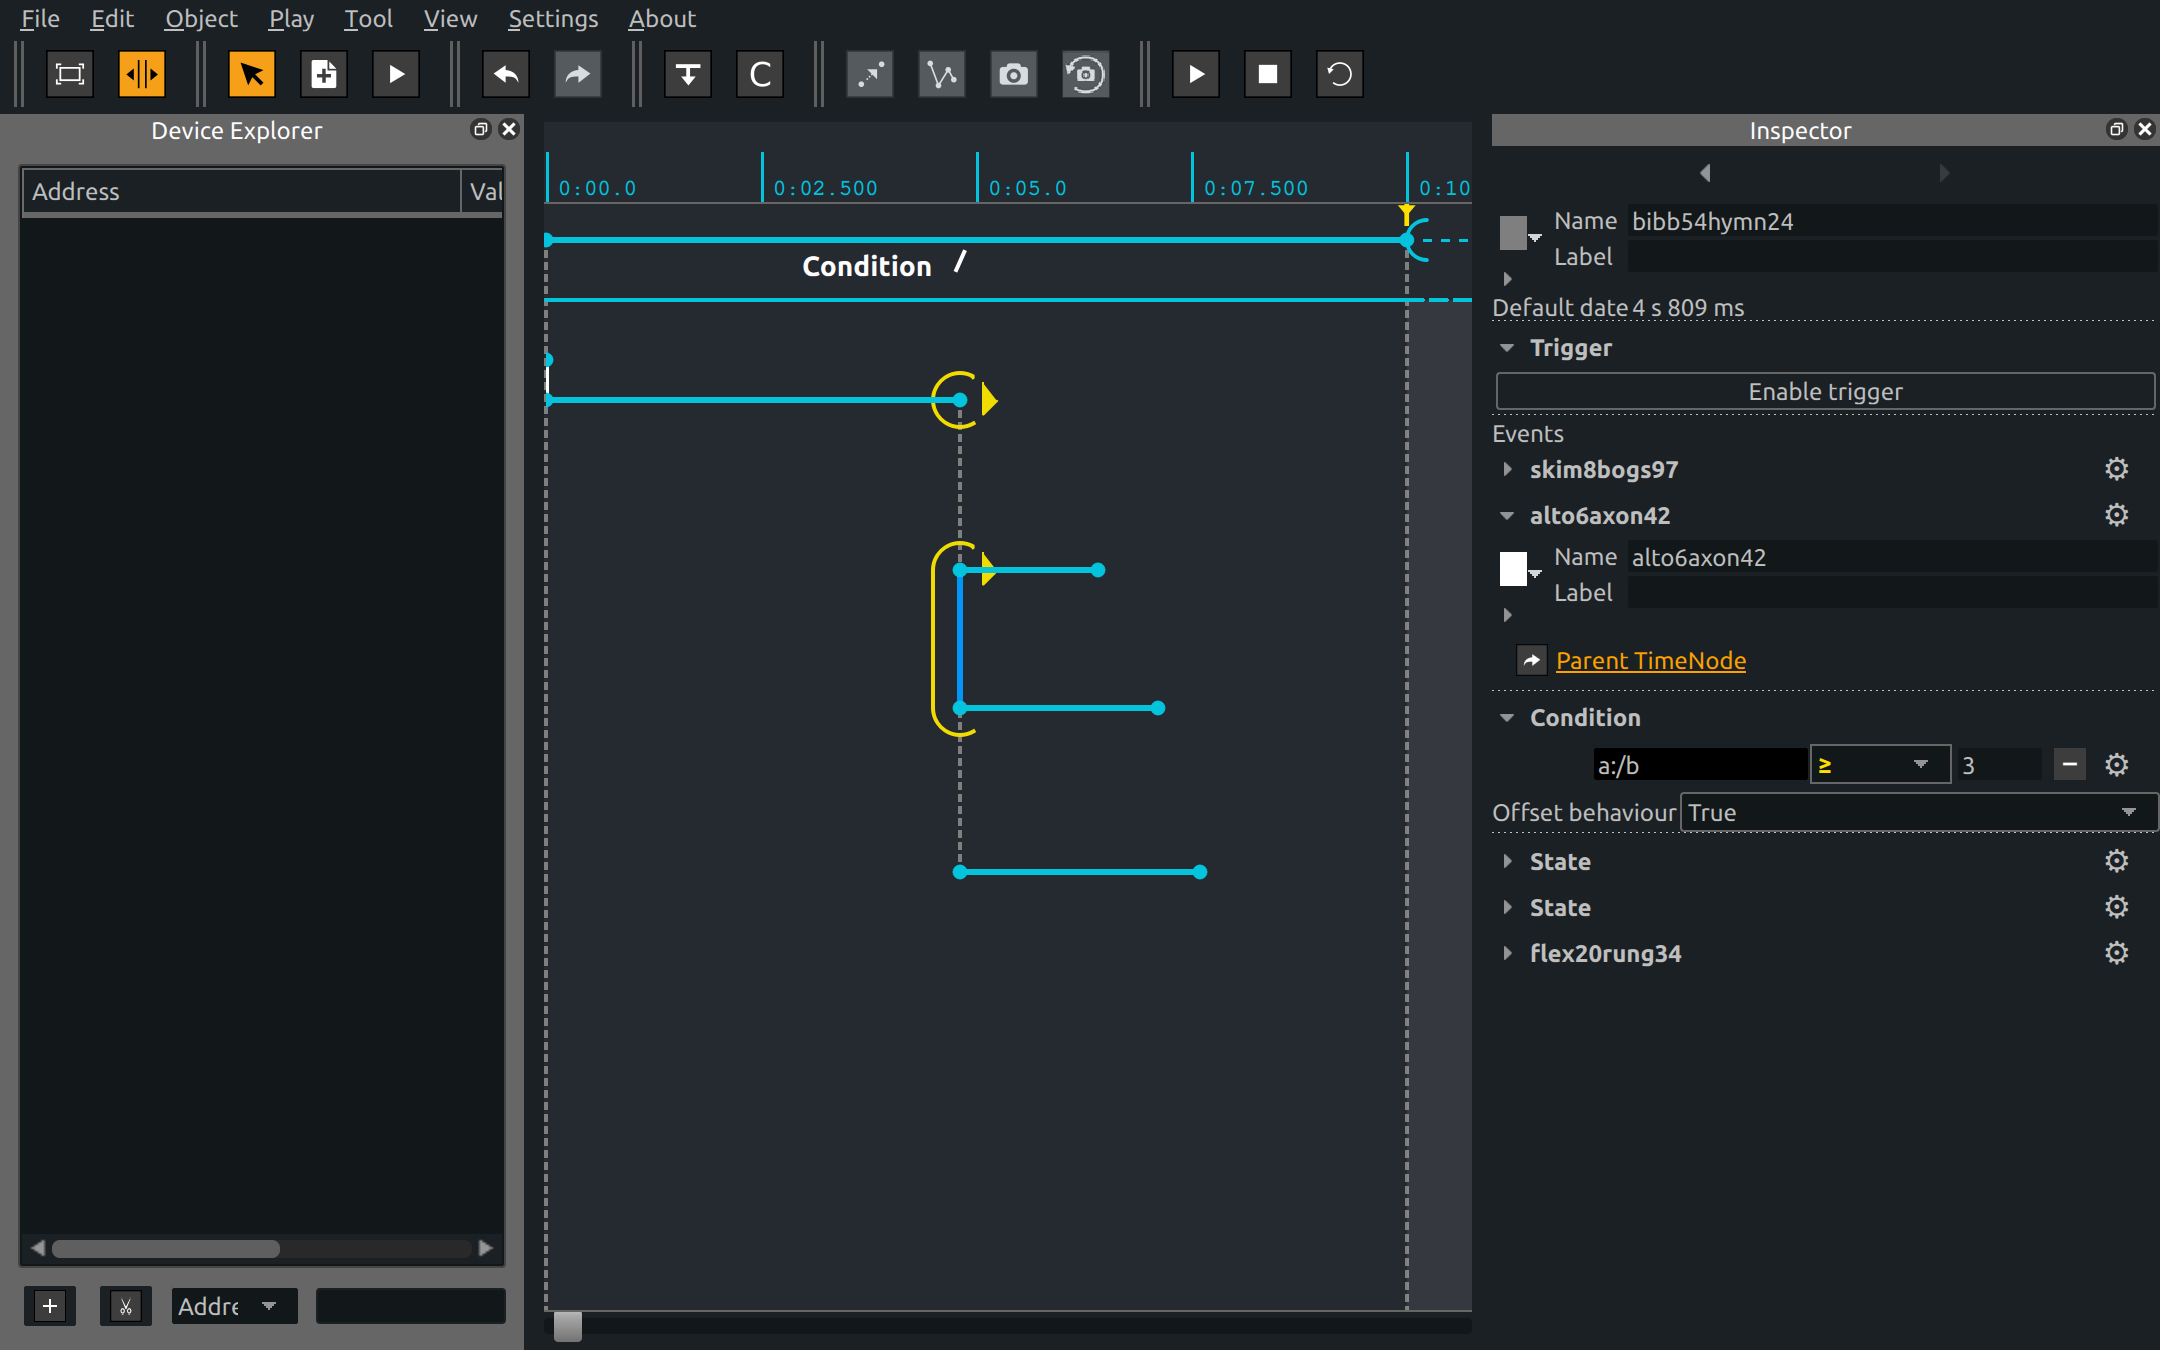
\includegraphics[width=\textwidth]{images/conditions.png}
\end{figure}
\end{frame}

\begin{frame}
\frametitle{Interactivity: trigger points}
\Large
\begin{figure}
    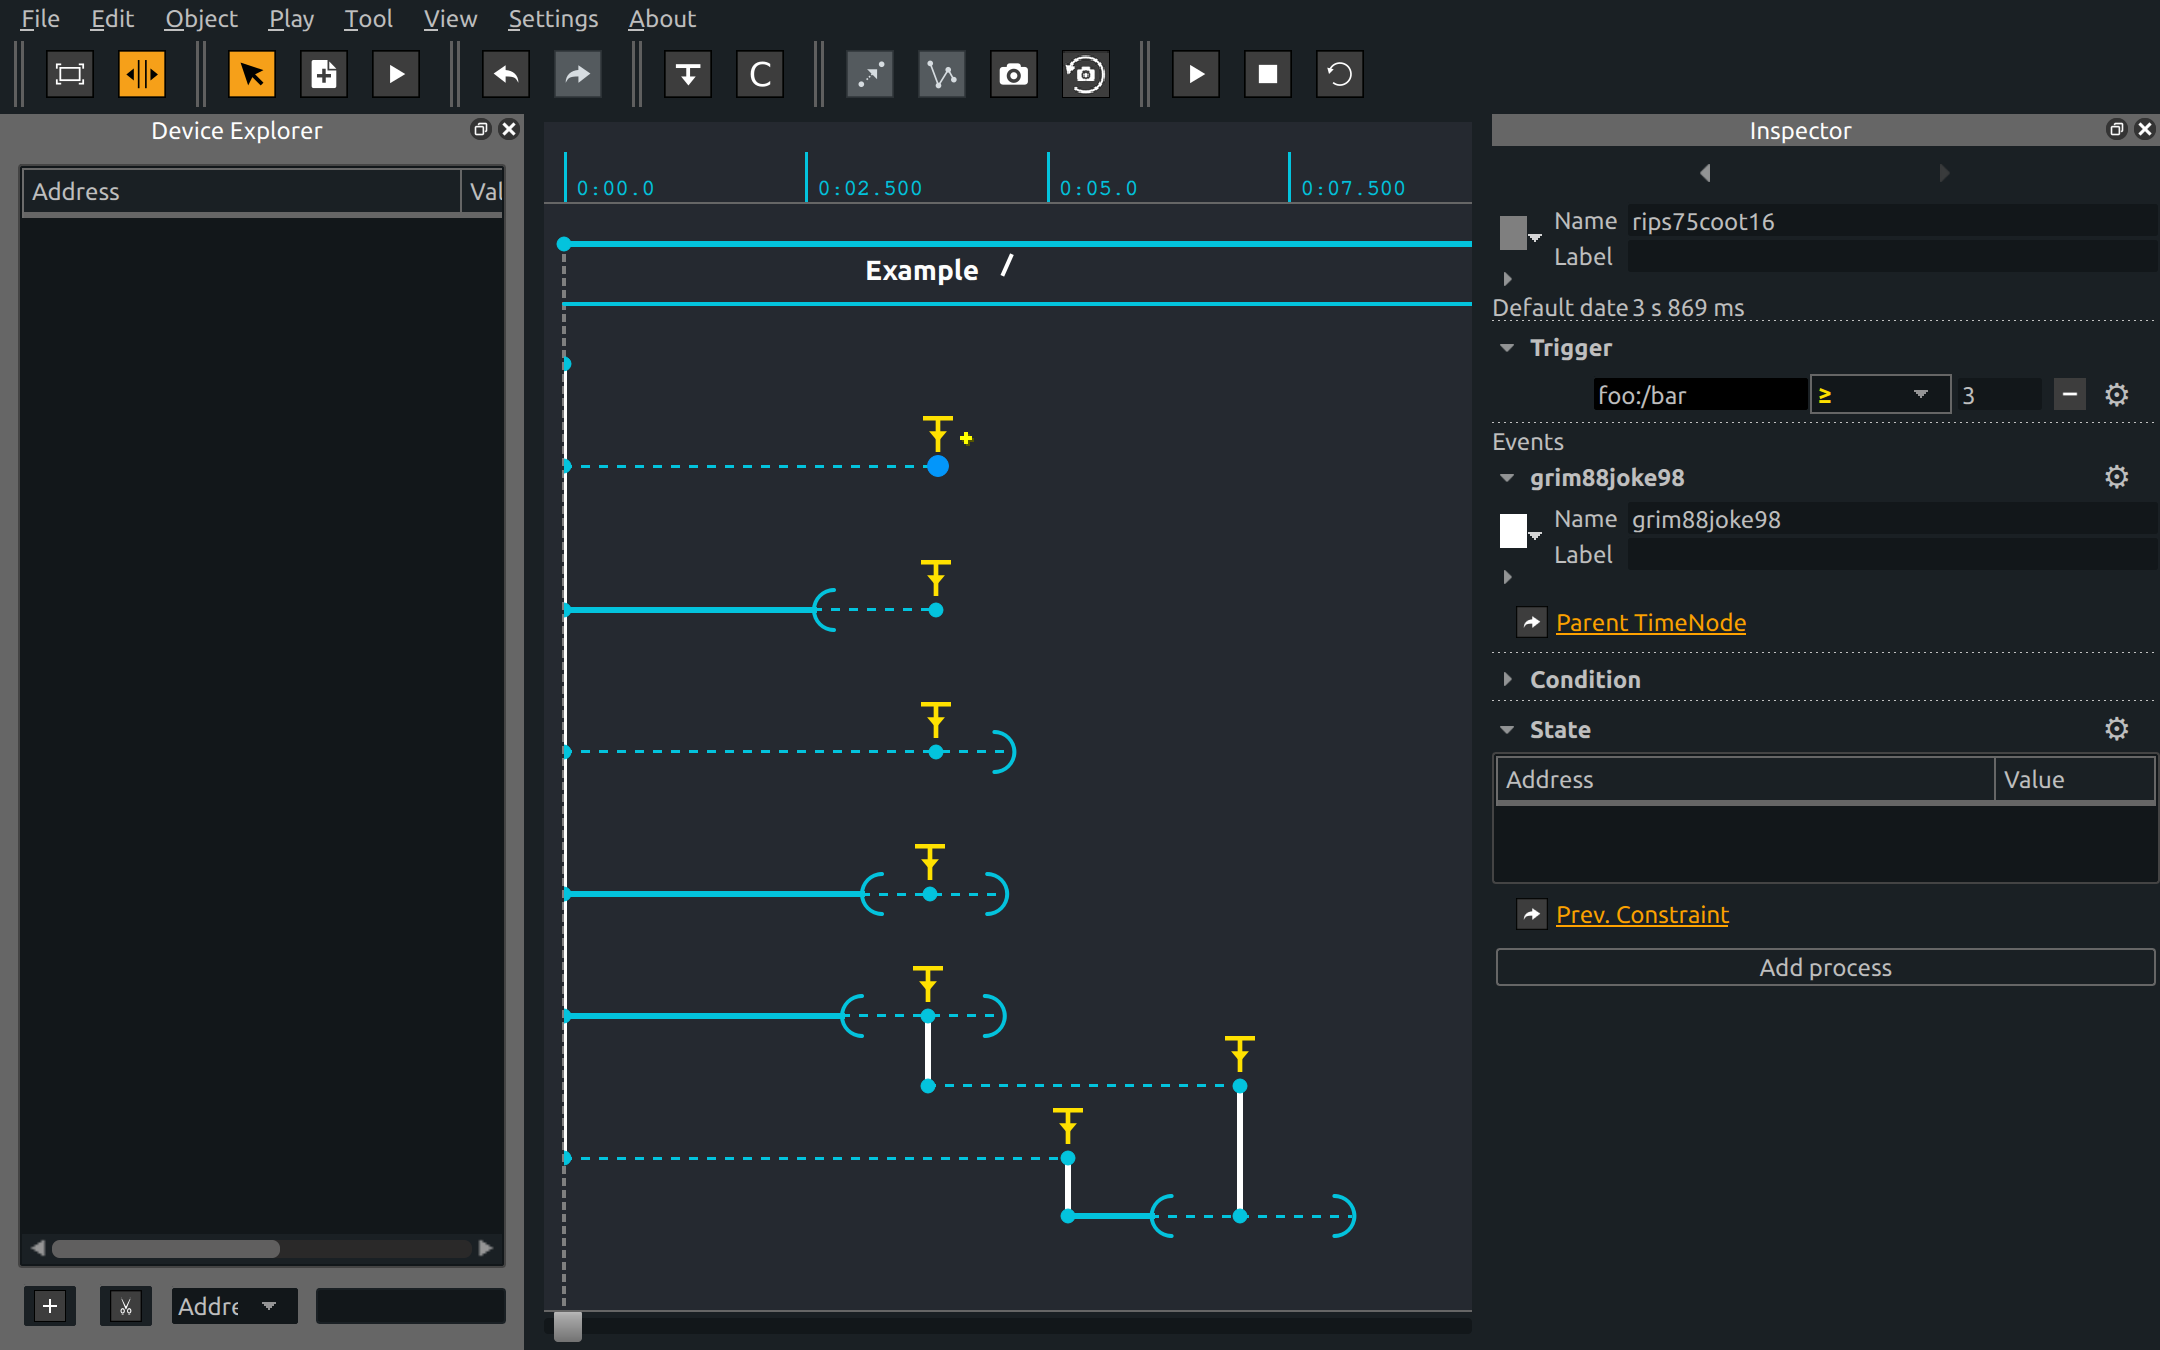
\includegraphics[width=\textwidth]{images/triggers.png}
\end{figure}
\end{frame}

\begin{frame}
\frametitle{Interactivity: execution speed}
\Large
\begin{figure}
    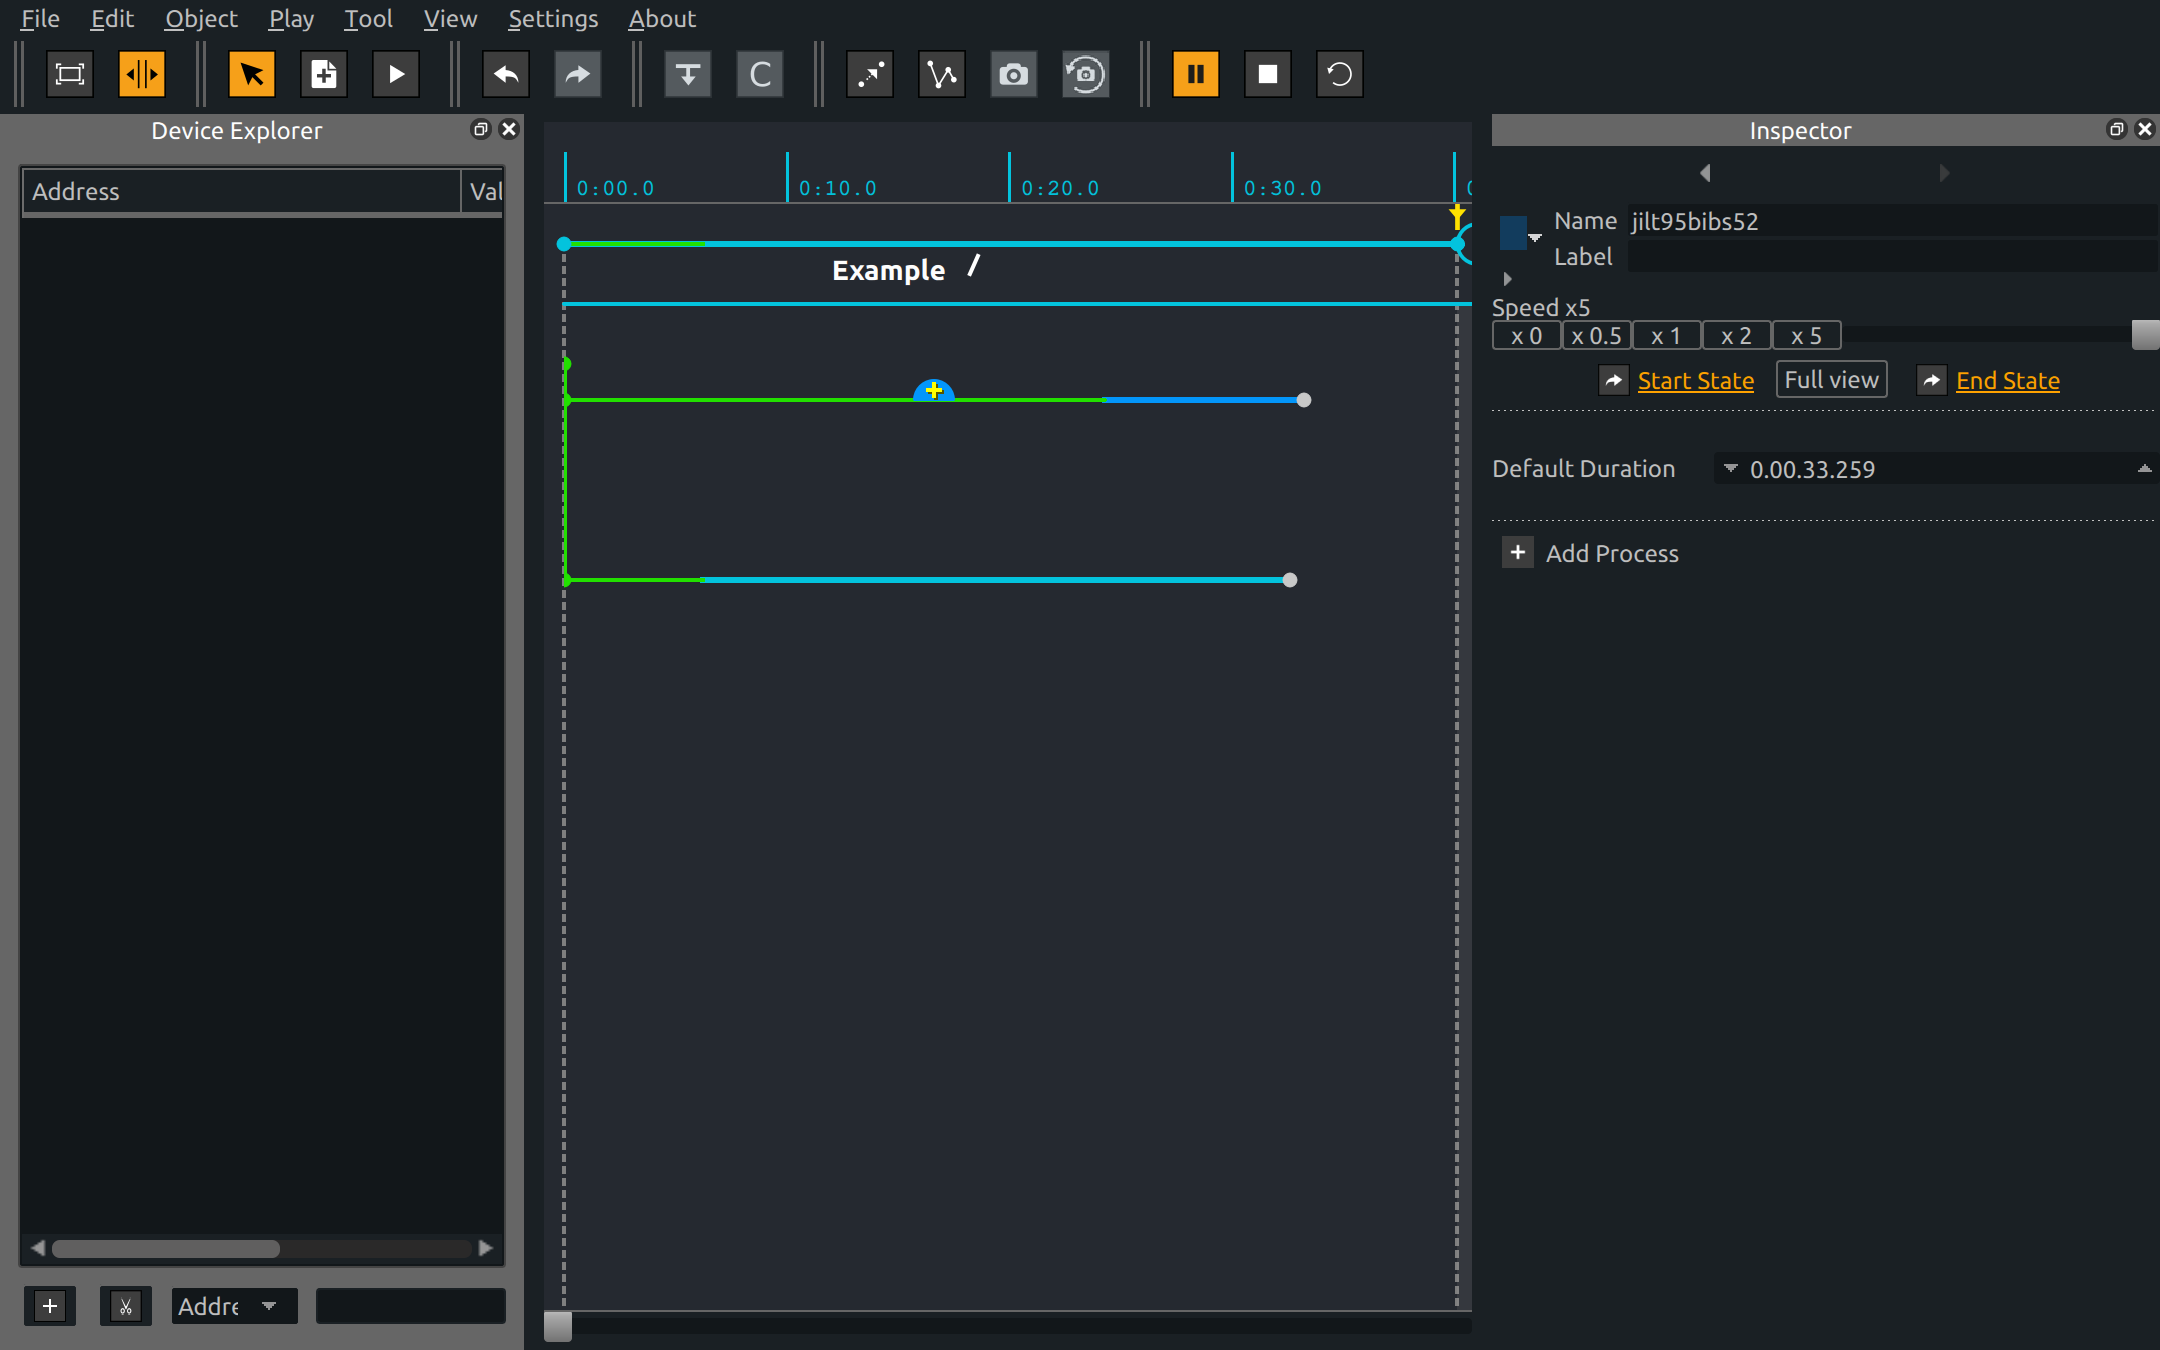
\includegraphics[width=\textwidth]{images/speed.png}
\end{figure}
\end{frame}

\subsection{Devices}
\begin{frame}
\frametitle{Working with external devices}
\Large
\begin{itemize}
    \item<1> Manual entry
    \item<2> Loading
    \item<3> Learning
    \item<4> Automatic discovery
\end{itemize}
\end{frame}

\begin{frame}
\centering
\Huge Demonstration
~\\
\Large MIDI control surface and WebSockets
\end{frame}

\section{Audio features}
\begin{frame}
\frametitle{Audio}
\Large
Hierarchical mixing, sounds, effects (Faust, LV2), sends...
\begin{figure}
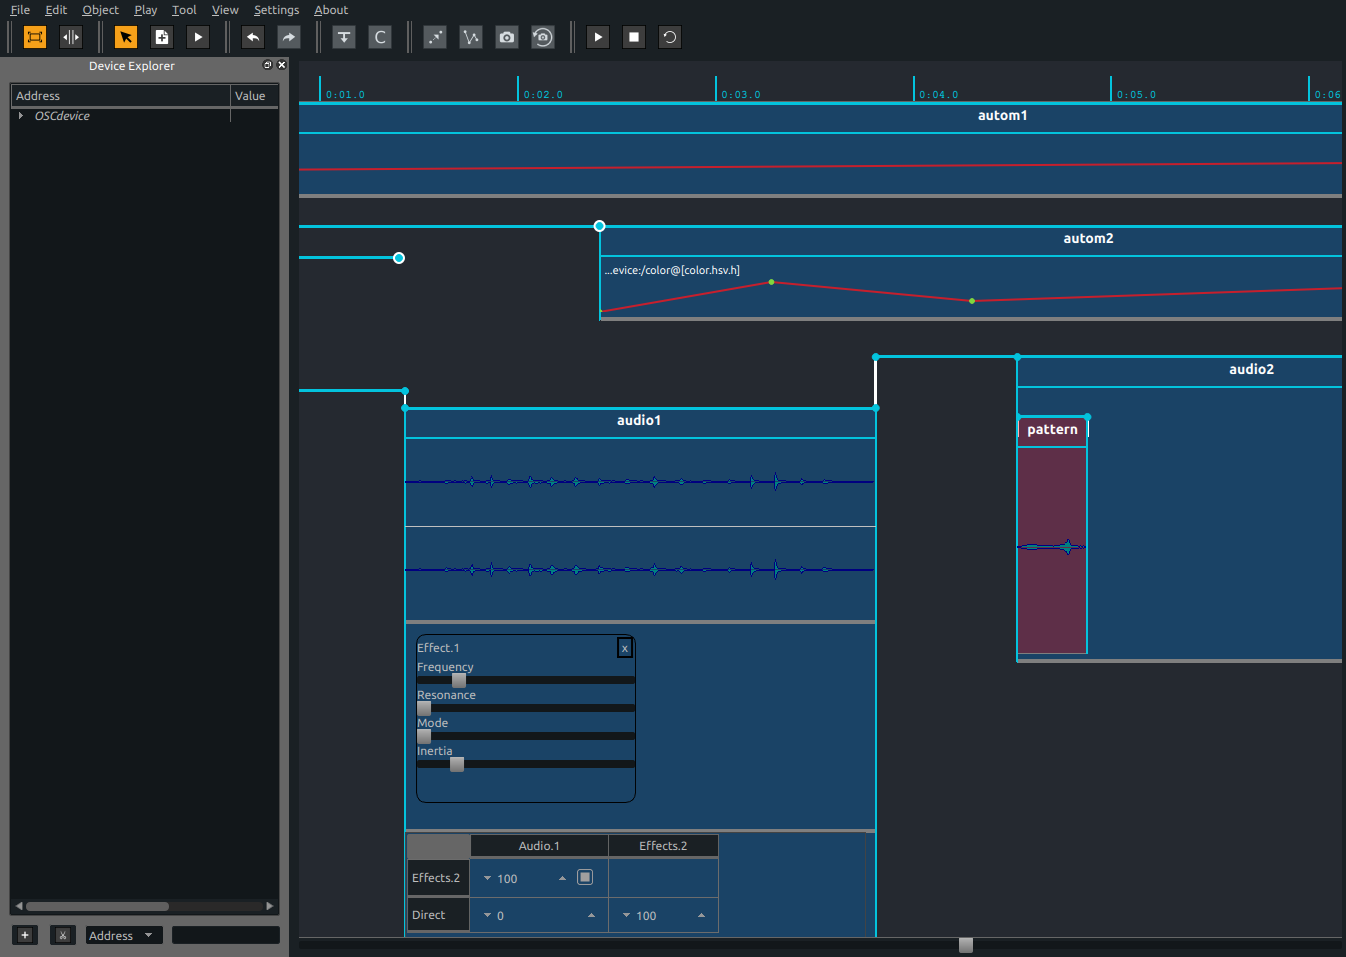
\includegraphics[width=0.8\textwidth]{images/audio.png}
\end{figure}
\end{frame}

\begin{frame}
\Large
\centering
The whole audio sequencing part is implemented with the plug-in API.
\end{frame}

\section{Conclusion}

\begin{frame}
\frametitle{What's missing}
\Large
\begin{itemize}
    \item<1> Multichannel operation.
    \item<2> Displaying LV2 UIs...
    \item<3> Musical time structures (bars, metronome, etc).
    \item<4> {\Huge \setsansfont{Symbola} 🙏} Packaging for distros {\Huge \setsansfont{Symbola} 🙏}
\end{itemize}
\end{frame}

\begin{frame}
\frametitle{Work-in-progress}
\Large
\begin{itemize}
    \item<1> Embedded score player.
    \item<2> Network operation.
    \item<3> Full-fledged audiograph.
    \item<4> Ongoing work on UI.
\end{itemize}
\end{frame}

\section{Workshop}

\begin{frame}
\frametitle{Workshop}
\Large
\begin{itemize}
    \item Building scores.
    \item Experimenting with your favorite environments.
    \item Gather your remarks and advices !
\end{itemize}
\end{frame}

\end{document}
